\documentclass[legal,11pt]{article}

\usepackage{wrapfig,graphics,graphicx}
\usepackage{array}
\usepackage{lscape}
\usepackage{graphicx}
\usepackage{ulem}
\usepackage{url}
\usepackage{threeparttable}
\usepackage{xcolor}
\usepackage{soul}
\usepackage{booktabs}
\usepackage[]{natbib}
\usepackage{amsmath}
\usepackage[colorlinks, linkcolor=red, anchorcolor=green, citecolor=blue]{hyperref}
%\graphicspath{{}{figures/}}
\usepackage{txfonts}
\usepackage{threeparttable}
\usepackage[document]{ragged2e}
\usepackage{multicol}


\oddsidemargin=-0.54cm
\evensidemargin=-0.54cm
\topmargin=-1in
\textwidth=17cm
\textheight=25cm
\pagestyle{empty}



%%========= Comments
\def\purple#1   {{\textcolor{purple}{#1}}\ }
\def\red#1    {\textcolor{red}{#1}}
\def\blue#1    {\textcolor{blue}{#1}}

\newcommand{\nbar}{\overline{n}}

\def\new#1    {{\bf #1 }}
\def\cut#1    {\sout{#1} }

%%========= Units
\def\kms    {\ifmmode{{\rm \ts km\ts s}^{-1}}\else{\ts km\ts s$^{-1}$}\fi}
\def\kms    {km\,s$^{-1}$\,}
\def\kmspc  {km\,s$^{-1}$pc$^{-1}$}
\def\arcsec {\hbox{$^{\prime\prime}$}}
\def\arcmin {\hbox{$^{\prime}$}}
\def\cmt   {cm$^{-3}$\,}
%\def\cmt   {cm$^{-3}$}
\def\Kcmt  {K\ cm$^{-3}$}
\def\Kkms{K\,\kms }
\def\Kkmspc{K\,\kms pc$^2$}
\def\jykms{Jy\,\kms }
\def\,{\thinspace}
\def\Msun{$M_\odot$}
\def\msun{$M_\odot$}
\def\Lsun{$L_\odot$}
%\def\hcnft{HCN$J= 4 \rightarrow 3$}
\def\hcopft{HCN$J= 4 \rightarrow 3$}
\def\HI{H{\sc i}}
\def\Htwo{H$_2$}
\def\MHtwo{$M_{\rm H_2}$}
\def\Tkin{$T_{\rm kin}$}
\def\to{$\rightarrow$}
\def\mum{$\mu$m}
\def\Tmb {$T_{\rm mb}$}
\def\Tsys {$T_{\rm sys}$}




\def\Lcsff  {$L'_{\rm CS\, J=5-4}$}
\def\Lcs    {$L'_{\rm CS}$}
\def\Lline  {$L'_{\rm line}$}





\def\nHtwo{$n({\rm H}_2)$}
\def\ncrit{$n_{\rm crit}$}

\def\LIR     {$L_{\rm IR}$}
\def\LCO     {$L_{\rm CO}$}
\def\LTIR     {$L_{\rm TIR}$}
\def\LFIR     {$L_{\rm FIR}$}
\def\Lgas    {$L'_{\rm gas}$}
\def\LHCNft  {$L'_{\rm HCN\, J=4-3}$}
\def\LHCNtt  {$L'_{\rm HCN\, J=3-2}$}
\def\LHCNoz  {$L'_{\rm HCN\, J=1-0}$}


\def\LHCOPft  {$L'_{\rm HCO^+\, J=4-3}$}
\def\LHCOP    {$L'_{\rm HCO^+}$}


\def\LCSss    {$L'_{\rm CS\, J=7-6}$}
\def\LCOtt    {$L'_{\rm CO\, J=3-2}$}
\def\LCOoz    {$L'_{\rm CO\, J=1-0}$}

\def\COtt    {CO$J=3-2$}


%%====== Molecular transitions
\def\xe         {$x_{\rm e}$}
\def\ne         {$n_{\mathrm{e}}$}
\def\nht        {$n_{\mathrm{H}_2}$}
\def\HCOP       {HCO$^{+}$}
\def\C2H        {C$_{2}$H}
\def\HC3N       {HC$_{3}$N}
\def\H2O        {H$_2$O}
\def\Htwo       {H$_2$}
\def\cCOoz      {$^{12}$CO\,$J$=1$\rightarrow$0 }
\def\cCOto      {$^{12}$CO\,$J$=2$\rightarrow$1 }
\def\cCOtt      {$^{12}$CO\,$J$=3$\rightarrow$2 }
\def\cCOft      {$^{12}$CO\,$J$=4$\rightarrow$3 }
\def\cCOsf      {$^{12}$CO\,$J$=6$\rightarrow$5 }
\def\cCOss      {$^{12}$CO\,$J$=7$\rightarrow$6 }
\def\ctCOoz     {$^{13}$CO\,$J$=1$\rightarrow$0 }
\def\ctCOto     {$^{13}$CO\,$J$=2$\rightarrow$1 }
\def\ctCOtt     {$^{13}$CO\,$J$=3$\rightarrow$2 }
\def\cci        {\ci $^{3}$P$_{1}\rightarrow^{3}$P$_{0}$\ }
\def\ci         {C\,{\sc i}\,}
\def\HCNoz      {HCN\,$J$=1$\rightarrow$0}
\def\HCOPoz      {HCO$^+$\,$J$=1$\rightarrow$0}
\def\HCOPtt      {HCO$^+$\,$J$=3$\rightarrow$2}
\def\CSto        {CS(J=2$\rightarrow$1)\ }
\def\HCNft        {HCN\,$J$=4$\rightarrow$3}
\def\HCNtt        {HCN\,$J$=3$\rightarrow$2}
\def\HCOPft     {HCO$^+\,J$=4$\rightarrow$3}
\def\CSss          {CS\,$J$=7$\rightarrow$6}
\def\CSff          {CS\,$J$=5$\rightarrow$4}
\def\COoz      {$^{12}$CO$J$=1$\rightarrow$0}
\def\COto      {$^{12}$CO$J$=2$\rightarrow$1}
\def\COtt      {$^{12}$CO$J$=3$\rightarrow$2}
\def\COft      {$^{12}$CO$J$=4$\rightarrow$3}
\def\COsf      {$^{12}$CO$J$=6$\rightarrow$5}
\def\COss      {$^{12}$CO$J$=7$\rightarrow$6}
\def\tCOoz     {$^{13}$CO$J$=1$\rightarrow$0}
\def\tCOto     {$^{13}$CO$J$=2$\rightarrow$1}
\def\tCOtt     {$^{13}$CO$J$=3$\rightarrow$2}
\def\cCOoz     {$^{12}$CO$J$=1$\rightarrow$0}
\def\cCOto     {$^{12}$CO$J$=2$\rightarrow$1}
\def\cCOtt     {$^{12}$CO$J$=3$\rightarrow$2}
\def\cCOft     {$^{12}$CO$J$=4$\rightarrow$3}
\def\cCOsf     {$^{12}$CO$J$=6$\rightarrow$5}
\def\cCOss     {$^{12}$CO$J$=7$\rightarrow$6}
\def\ctCOoz    {$^{13}$CO$J$=1$\rightarrow$0}
\def\ctCOto    {$^{13}$CO$J$=2$\rightarrow$1}
\def\ctCOtt    {$^{13}$CO$J$=3$\rightarrow$2}
\newcommand{\sigmadense}{$\Sigma_\text{dense}$}
\newcommand{\fdense}{$f_\text{dense}$}
\newcommand{\sigmasfr}{$\Sigma_\text{SFR}$}
\newcommand{\sigmastellar}{$\Sigma_\text{stellar}$}
\newcommand{\sfedense}{SFE$_\text{dense}$}


%%%BIB
\def\aj{AJ}%
          % Astronomical Journal
\def\actaa{Acta Astron.}%
          % Acta Astronomica
\def\araa{ARA\&A}%
          % Annual Review of Astron and Astrophys
\def\apj{ApJ}%
          % Astrophysical Journal
\def\apjl{ApJ}%
          % Astrophysical Journal, Letters
\def\apjs{ApJS}%
          % Astrophysical Journal, Supplement
\def\ao{Appl.~Opt.}%
          % Applied Optics
\def\apss{Ap\&SS}%
          % Astrophysics and Space Science
\def\aap{A\&A}%
          % Astronomy and Astrophysics
\def\aapr{A\&A~Rev.}%
          % Astronomy and Astrophysics Reviews
\def\aaps{A\&AS}%
          % Astronomy and Astrophysics, Supplement
\def\azh{AZh}%
          % Astronomicheskii Zhurnal
\def\baas{BAAS}%
          % Bulletin of the AAS
\def\bac{Bull. astr. Inst. Czechosl.}%
          % Bulletin of the Astronomical Institutes of Czechoslovakia 
\def\caa{Chinese Astron. Astrophys.}%
          % Chinese Astronomy and Astrophysics
\def\cjaa{Chinese J. Astron. Astrophys.}%
          % Chinese Journal of Astronomy and Astrophysics
\def\icarus{Icarus}%
          % Icarus
\def\jcap{J. Cosmology Astropart. Phys.}%
          % Journal of Cosmology and Astroparticle Physics
\def\jrasc{JRASC}%
          % Journal of the RAS of Canada
\def\mnras{MNRAS}%
          % Monthly Notices of the RAS
\def\memras{MmRAS}%
          % Memoirs of the RAS
\def\na{New A}%
          % New Astronomy
\def\nar{New A Rev.}%
          % New Astronomy Review
\def\pasa{PASA}%
          % Publications of the Astron. Soc. of Australia
\def\pra{Phys.~Rev.~A}%
          % Physical Review A: General Physics
\def\prb{Phys.~Rev.~B}%
          % Physical Review B: Solid State
\def\prc{Phys.~Rev.~C}%
          % Physical Review C
\def\prd{Phys.~Rev.~D}%
          % Physical Review D
\def\pre{Phys.~Rev.~E}%
          % Physical Review E
\def\prl{Phys.~Rev.~Lett.}%
          % Physical Review Letters
\def\pasp{PASP}%
          % Publications of the ASP
\def\pasj{PASJ}%
          % Publications of the ASJ
\def\qjras{QJRAS}%
          % Quarterly Journal of the RAS
\def\rmxaa{Rev. Mexicana Astron. Astrofis.}%
          % Revista Mexicana de Astronomia y Astrofisica
\def\skytel{S\&T}%
          % Sky and Telescope
\def\solphys{Sol.~Phys.}%
          % Solar Physics
\def\sovast{Soviet~Ast.}%
          % Soviet Astronomy
\def\ssr{Space~Sci.~Rev.}%
          % Space Science Reviews
\def\zap{ZAp}%
          % Zeitschrift fuer Astrophysik
\def\nat{Nature}%
          % Nature
\def\iaucirc{IAU~Circ.}%
          % IAU Cirulars
\def\aplett{Astrophys.~Lett.}%
          % Astrophysics Letters
\def\apspr{Astrophys.~Space~Phys.~Res.}%
          % Astrophysics Space Physics Research
\def\bain{Bull.~Astron.~Inst.~Netherlands}%
          % Bulletin Astronomical Institute of the Netherlands
\def\fcp{Fund.~Cosmic~Phys.}%
          % Fundamental Cosmic Physics
\def\gca{Geochim.~Cosmochim.~Acta}%
          % Geochimica Cosmochimica Acta
\def\grl{Geophys.~Res.~Lett.}%
          % Geophysics Research Letters
\def\jcp{J.~Chem.~Phys.}%
          % Journal of Chemical Physics
\def\jgr{J.~Geophys.~Res.}%
          % Journal of Geophysics Research
\def\jqsrt{J.~Quant.~Spec.~Radiat.~Transf.}%
          % Journal of Quantitiative Spectroscopy and Radiative Trasfer
\def\memsai{Mem.~Soc.~Astron.~Italiana}%
          % Mem. Societa Astronomica Italiana
\def\nphysa{Nucl.~Phys.~A}%
          % Nuclear Physics A
\def\physrep{Phys.~Rep.}%
          % Physics Reports
\def\physscr{Phys.~Scr}%
          % Physica Scripta
\def\planss{Planet.~Space~Sci.}%
          % Planetary Space Science
\def\procspie{Proc.~SPIE}%
          % Proceedings of the SPIE





\begin{document}

\begin{center}
        {\large\bf Mapping the Dense Molecular Gas in the Strongest Star-forming Galaxies}

%CS 2-1/3-2 mapping along the major axes of nearby gas-rich galaxies}

%HARP HCN/HCO+(4-3)/CS(7-6) mapping in ~20 strongest nearby SF gals/starbursts
\vspace { 0.5 cm}
 {\Large\bf Abstract} 
\justify
{{
This new proposal builds upon the existing JCMT MALATANG survey (nearly 400 hrs) and
the IRAM EMPIRE survey (~600hrs) will tackle the complex issues on the dense gas 
excitation by focusing on the analysis of multi-ladder and multi-line. 

We propose additional observing time to expand our MALATANG program to construct 
the largest and deepest \HCNft\ and \HCOPft\ (the strongest collisionally excited 
molecular lines after CO) maps in a complete infrared (IR) flux limited sample of 23
brightest IR galaxies plus 5 additional IR-bright galaxies in the EMPIRE survey. 
The EMPIRE survey consists of a total of 9 galaxies with 4 galaxies already observed in
our MALATANG program. Combining two surveys, the detailed studies on the excitation will be available beyond
the central beam on the nuclear regions.

%%%%%
Previous $\sim$ 600 hrs observations with the IRAM 30m lead to a large \HCNoz\ and \HCOPoz{}\  maps
in nearby star-forming galaxies, demonstrating the large-scale extended distribution of dense molecular 
gas beyond the nuclear $\sim$ kpc regions in spiral galaxies. The HARP-B array on 
the JCMT provides the unique mapping machinery in studying the dense gas excitation, 
chemistry, probing even denser and warmer gas at close to the peak ladder in the 
spectral line energy distribution in these molecular lines.  This survey will help 
shed fundamental new light on how the molecular gas forms stars on different 
physical scales and under various physical environments.  The survey will offer a unique
database, via diagnostic power of various line ratios (HCN, \HCOP\ \& CO),  for 
connecting the emissions between dense molecular gas tracers and star formation (SF) 
in both central cores of galaxies and more extended regions in spiral disks. 
%%%%%

Combining with our ongoing efforts with the JCMT and other telescopes and the 
rich data in literature, this survey will also raise the opportunity to tackle 
many scientific issues including the initial conditions of SF, chemistry, kinematics,
feedback of SF and AGN, excitation conditions of molecules, as well as the connections 
between SF and dense molecular gas on various physical scales. 

Our MALATANG sample was a complete flux-limited sample of IRAS Revised Bright Galaxy survey
with $f_{\rm 60\mu m}>$ 50 Jy and $f_{\rm 100\mu m}>$ 100 Jy.  In this proposal, we plan to extend MALATANG to map 
\HCNft\ and \HCOPft\ along the major axes of 6 EMPIRE galaxies including a JIGGLE map in M51.
The planed observations will reach to a sensitivity of 0.3 \Kkms ($\sim$4.5$\times10^6$ \Msun)
per beam, with a linear resolution from 0.2 to 2.8 kpc.  

The final survey sample will consist of 23 nearest and brightest infrared galaxies plus 5 IR-bright galaxies beyond
the local group that already have  extremely abundant legacy data from ground to space and needs a modest $\sim$270 hrs band 3 time (some portions can be observed under weather bands 2 and 4 and they are also estimated for each) to complete.  This will be {\bf the first systematic dense gas mapping survey in the off-central regions of nearby galaxies}. }}

\end{center}


\begin{table}[htbp]

\centering
{List of co-Is}
\small
\addtolength{\tabcolsep}{-1.pt}

\begin{threeparttable}[b]
\begin{tabular}{lcclcc}
\hline
\hline

Name & Affiliation & Country & Name & Affiliation & Country \\

\hline

Kotaro Kohno         & U. Tokyo          & JP & Toby Moore   & Liverpool John Moores U.  & UK \\  
Masa Imanishi        & NAOJ              & JP & Stephen Serjeant  & Open U.       & UK \\ 
Daisuke Iono         & NAOJ              & JP & Jeff Wagg         & SKA Org.      & UK \\
Quang Nguyen Luong   & NAOJ              & JP & Christine Wilson  & McMaster U.   & CA \\
Kouichiro Nakanishi  & NAOJ              & JP & Erik Rosolowsky   & U. Alberta    & CA \\
Sherry C. C. Yeh     & NAOJ              & JP & Scott Chapman     & Dalhousie U.  & CA \\
Joanna Bulger        & NAOJ              & JP & Kevin Lacaille.   & Dalhousie U.  & CA \\ 
Keiichi Maeda        & Kyoto U.          & JP & Ashley Bemis      & McMaster U.   & CA  \\
Yusuke Miyamoto      & Nobeyama          & JP & Richard de Grijs  & Macquarie U.  & AU \\
Tomoka Tosaki        & Joetsu U. of Edu. & JP & Sarah Graves      & EAO           & US \\
An-Li Tsai           & NCU               & TW & Harriet Parsons   & EAO           & US  \\
Nanase Harada        & ASIAA             & TW & Mark G. Rawlings  & EAO           & US  \\
Satoki Matsushita    & ASIAA             & TW & L. Cheng          & THU           & CN \\ 
Hsi-An Pan           & ASIAA             & TW & J.-Z. Wang        & SHAO          & CN  \\
Yujin Yang           & KASI              & KR & T. Xiao           & ZJU           & CN \\ 
Minjin Kim           & KASI              & KR & Y.-X. Xie         & PKU           & CN \\
Hong Soo Park        & KASI              & KR & J.-Y. Shangguan   & PKU           & CN \\
Aeree Chung          & Yonsei U.         & KR &  H. Gao           & PKU           & CN \\
Bumhyun Lee          & Yonsei U.         & KR & Yali Shao         & PKU           & CN \\
Sungeun Kim          & Sejong U.         & KR & S.-Y. Yu          & PKU           & CN \\
Soojong Pak          & Kyung Hee U.      & KR & Luis C. Ho        & PKU           & CN \\
Hye-In Lee           & Kyung Hee U.      & KR & Y.-X. Xie         & PKU           & CN \\
Padelis Papadopoulos & Cardiff U.        & UK & Y. Shi            & NJU           & CN \\ 
Walter Gear          & Cardiff U.        & UK & H. Chen           & NJU           & CN \\
Haley Gomez          & Cardiff U.        & UK & B. Jiang          & NJU           & CN \\
Chris Clark          & Cardiff U.        & UK & J.-J. Qiu         & NJU           & CN \\
Andrew Rigby         & Cardiff U.        & UK & Q.-S. Gu          & NJU           & CN \\
Matt Smith           & Cardiff U.        & UK & T.-T. Fang.       & XMU           & CN \\
Loretta Dunne        & Cardiff U.        & UK & J.-F. Wang        & XMU           & CN \\ 
Stephen Eales        & Cardiff U.        & UK & J.-W. Wu          & NAOC          & CN \\
Timothy A Davis      & Cardiff U.        & UK & M. Zhu            & NAOC          & CN \\
Serena Viti          & UCL               & UK & X.-H. Li          & NAOC          & CN \\
George Kelly         & UCL               & UK & J.-H. He          & YNAO          & CN \\
Amelie Saintonge     & UCL               & UK & Y.-H. Zhao        & YNAO          & CN \\
Richard Tunnard      & UCL               & UK & Y.-X. He.         & XAO           & CN \\
Malcolm Currie       & RAL               & UK & X.-J. Jiang       & PMO           & CN \\ 
Ilse Looze.          & UCL               & UK & Q.-H. Tan         & PMO           & CN \\
Elias Brinks         & U. Hertfordshire  & UK & Q. Jiao           & PMO           & CN \\
Kristen Coppin       & U. Hertfordshire  & UK & J.-F. Wang.       & PMO           & CN \\
GiuLio Violino       & U. Hertfordshire  & UK & Y.-P. Ao          & PMO           & CN \\
Mark Sargent         & U. Sussex         & UK & H.-J. Ma          & PMO           & CN \\
Dimitra Rigopoulou   & U. Oxford         & UK & C.-T. Yang        & PMO           & CN \\
Michal Michalowski   & U. Edinburgh.     & UK & D.-Z. Liu         & PMO           & CN \\
John Richer          & U. Cambridge      & UK & L.-J. Liu         & PMO           & CN \\
David Eden           & Liverpool John Moores U.  & UK & \\ 

\hline
\end{tabular}
 
\begin{tablenotes}[para,flushleft]
{\bf Co-PIs: Yu Gao (PMO, CN), Zhiyu Zhang (NJU, CN), Thomas Greve (UCL, UK)}\\
\end{tablenotes}
\end{threeparttable}

\end{table}


%-------------------------------------------------------------------

\clearpage
\justify
\medskip


\section{Background and Motivation:}

\subsection{Dense Molecular Gas --- Key to Star Formation }


The star formation (SF) process constantly turns gas into stars and drives 
galaxy formation and evolution. It is, however, not yet fully understood how 
gas properties affect the ability to form stars. Questions which naturally arise
are: Which phases of gas are directly connected to SF, what kind of physical
processes regulate SF and its feedback, and is there a universal physical law
applying for all types of SF and all kinds of galaxies near and far?   


Based on observations of CO and \HI, which trace molecular (\Htwo) and atomic
gas respectively, the Kennicutt-Schmidt (K-S) law relates the global
surface-densities of SF rate ($\Sigma_{\rm SFR}$) and total amount of neutral
gas ($\Sigma$gas :\HI + \Htwo) in star-forming galaxies by introducing a super
linear exponent, $\alpha \sim 1.4 ~ (\Sigma_{\rm SFR} \propto \Sigma_{\rm
gas}^\alpha)$ \citep{Kennicutt2012}. This empirical relationship connects total
gas and SF, but the super linear $\alpha$ indicates a non-constant SF
efficiency increases with  different SF rate, traced by infrared (IR)
luminosity \LIR. Quite a range of deviation from the K-S law, however, has also
been found in different types of galaxy samples, both in global and in
spatially resolved studies with (sub)kpc resolutions
\citep[e.g.,][]{Kennicutt2012,Bigiel2008}.  


With high spatial resolution and large scale mapping observations of \COto\ and
\HI\ in nearby normal spiral galaxies, it is found that \HI\ is not related to
SF \citep[e.g.,][]{Bigiel2008}. For the \Htwo\ gas traced by low-$J$ ($J\le2$)
CO emission, SF is nearly linearly correlated with \Htwo, in the disks of local
spiral galaxies even to the extended \HI\ dominated outer disk
regions (e.g., \citealt{Bigiel2008,Schruba2011,Leroy2013}). This linearity,
however, only holds in a very narrow range of surface density of SF and on
physical scales greater than 200 pc.  Moreover, this relation becomes super
linear when starburst regions and extreme starbursts such as ultraluminous
IR galaxies (ULIRGs) are included (e.g.,
\citealt{Genzel2010,Daddi2010a}).  


The dense molecular gas (\nHtwo\ $\ge$ 10$^4$\cmt) stands out to have much
tighter and direct connection with SF than that of total gas (\HI + \Htwo) or
only \Htwo. \citet[][see Fig. \ref{fig:hcn10}]{gs04a,gs04b} have shown that 
galaxies exhibit a linear correlation between the far-IR and HCN $J$=1$\rightarrow$0 
luminosities, over three orders of magnitude range. These correlations even extend 
to dense cores in giant molecular clouds (GMCs) in the Milky Way \citep{weg05,zgh2014}.
These results imply that the dense gas is the gas phase that is forming
stars. The change of the slopes of the K-S relation in different galaxy samples
simply reflects the variation of the dense gas fraction \citep[e.g.,][]{Lada2010b}. 

Recent advances in our understanding of SF do suggest that active high-mass SF,
is {\it essentially and exclusively} formed in the dense cores of GMC
\citep[e.g.,][]{Evans08}. The dense gas tracers (e.g., HCN, HCO$^+$, CS etc. )
exhibit, beside CO, the strongest collisional excited lines in galaxies (e.g.,
\citealt{rwc06,gc08,Baan08,Greve14}), suggesting that the extremely high SF
efficiency found in ULIRGs simply reflects the tremendous amount of {\it dense}
molecular gas available, but not the total gas mass
content\citep[e.g.,][]{Lada2010b}.  More IR luminous galaxies tend to have
higher SF rate per unit total molecular mass, whereas the SF rate per unit
dense molecular mass is likely constant \citep[][]{gs04a,gs04b}.

\cite{lgg2015} have examined the relations between the galaxy averaged surface
densities of the various gas components (atomic, molecular, total gas, and
dense molecular gas) and SF rate in a sample of 181 local galaxies with IR
luminosities spanning $\sim$ five orders of magnitude. We have taken a novel
approach and used high-resolution radio continuum observations to measure
accurately the sizes of the areas of active SF within the galaxies, a key step
as it directly affects the surface densities of gas and SF. In our
sample, we find that the surface density of dense molecular gas (as traced by
HCN) has the tightest correlation with that of SF rates, and is linear in
log--log space (power-law slope of N = 1.01 $\pm$ 0.02) across the full galaxy
sample (see Fig. \ref{fig:hcn-ir}). The correlation between surface densities
of molecular gas (traced by CO) and $\Sigma_{\rm SFR}$ is sensitive to the
adopted value of the CO-to-H$_2$ conversion factor used to infer molecular gas
masses from CO luminosities. If instead we adopt conversion factor values  of
4.6 and 0.8 for disk galaxies and (U)LIRGs, respectively, we find the two
galaxy populations separate into two distinct $\Sigma_{\rm SFR}$  versus
$\Sigma_{\rm H2}$ relations. We find no correlation between global surface
densities of SF rates and atomic gas.

\subsection{General Properties of High Density Gas Tracers  }

The low-$J$ transitions ($J\le2$) of CO lines have critical densities of only
$\sim$ 300 - 1000 \cmt/$\tau$ \footnote{For multiple energy level molecular
system: $n_{\rm crit}={\Sigma_{\rm l<u} A_{\rm ul}}/{\Sigma_{\rm l\neq u}
C_{\rm ul}}$, or a given \Tkin\ \citep{Jansen1995, Osterbrock2006}.}, making them good
tracers of the mass of total \Htwo\ gas (\MHtwo). This density range matches
well with the bulk of the GMCs. However, such bulk of H$_2$ gas is not
forming stars everywhere.  Only the gas at high density in the dense cores has
sufficiently gravity to collapse and eventually form stars.  A physical
connection between the \Htwo\ gas density and SF is naturally expected, 
as this is where gravity dominates the turbulent pressure and magnetic force 
in clouds, leading to collapse and fragmentation and eventual formation of stars.



%The essential method to test this scenario is to perform synergetic
%observations of multiple molecular lines with different critical densities. 

By climbing up the \ncrit\ of  molecular gas tracers, we can gain insight into
the physics from the bulk of the molecular gas to the sites of on-going SF, and
further explore how the gas density affects SF process.  The rotational
transitions of the molecules with high dipole moments and high abundances by
number compared to that of hydrogen ($\sim 10^{-6}-10^{-8}$ relative to \Htwo;
e.g., HCN, \HCOP, CS, etc.), become the most common tracers of dense gas since
they are the most luminous molecular lines after CO and even observable in high
redshift. Detailed studies of HCN and \HCOP in bright, nearby galaxies can then
be useful
and much needed in extending our knowledge in the local Universe to
help interpret observations in galaxies at
high redshift.. The $J$=1--0
transition of these molecules have a \ncrit\  of $10^4 - 10^6$\cmt, which are
representative \Htwo\ density of Galactic dense cores
\citep[e.g.,][]{Plume1997,weg05}. 



For the $J$=1--0, 3--2, and 4--3 transitions of HCN,  \ncrit\ are $\sim$ 2
$\times 10^5$ \cmt, 5$\times 10^6$ \cmt, and 1.5 $\times 10^7$ \cmt, and upper
level energies are 4 K, 26 K, and 46 K, respectively. The high-$J$ transitions
are also less affected by the line trapping, so the effective \ncrit\ keeps
almost-uninfluenced by column density. So, the high-$J$ transitions probe {\bf very high density and relatively warm} cores, which are setting up the initial conditions of star-formation.
Because UV photons can not penetrate to Av$>$7-10, and turbulence dissipates quickly in dense regions, these dense molecular cores can only be heated up by cosmic rays and gravitational collapsing.  
High-$J$ ($J\ge 5$) CO transitions, on the other hand, also have high \ncrit. 
However, the high-$J$ CO lines also need very high kinetic temperature $\sim$hundreds of K to be excited efficiently. Thus, high-$J$ CO lines are 
the effects by star-formation, instead of the cause of it. The high-$J$ CO transitions are also difficult to
access from the ground while the HCN and \HCOP are readily available.




\subsection{Chemical Properties of High Density Gas Tracers  }

Through comparison with models, abundances of molecules tracing dense gas and
their line ratios can be used not only to infer the physical conditions of the
gas but also to constrain the chemical reactions that drive molecule formation
and destruction in irradiated regions\citep[e.g.,][]{vandishoeck1998}. Subject
to a proper interpretation, observations of molecular emission are extremely
sensitive to trace the material that is the reservoir or leftover of the star
formation process, as well as the process of star formation itself. Molecular
abundances can be interpreted through models for Photon-Dominated Regions
(PDRs), X-ray Dominated Regions (XDRs), Mechanical Dominated Regions (MDRs),
and are among the best diagnostics for disentangling star formation.

In general and on large scales, the overall abundance of molecules is
determined by the element abundances, physical conditions and
energetic processes, such as UV or X-ray radiation,  which in general tend to
destroy molecules.  The abundances of different molecules vary in different
physical environments, such as super wind from starbursts, strong radiation
from AGNs, jets and outflows, large scale shocks in merging activities, Cosmic
Rays, etc. Specifically, chemical processes between HCN, HNC, and CN could
change their abundances in different temperatures \citep{Baan08}. The ratios
between HCN and \HCOP\ could also be affected by chemical
complexities\citep[e.g.,][]{krips08}, ionization rates and electron densities
\citep[e.g.][]{PPP2007}, and shocks \citep[e.g.,][]{Xie95}. All above issues
make it difficult to find a stable dense gas tracer in the extreme environment
of galaxies. 

The use of molecules as diagnostics of different gas conditions stems from the
fact that different molecules {\it and} different transitions of the same
molecule will trace different regions of a galaxy from the cold, relatively low
density molecular gas (mostly traced by CO), to highly excited shock regions ( 
traced by e.g., SiO), and finally to very high density star forming clouds (traced by
e.g., HCN). Often high abundances of particular species such as HCO$^+$ are
automatically attributed to the presence of strong PDRs, since this molecule is
indeed abundant in the presence of a strong UV field, regardless of the
metallicity, cosmic ray ionisation rate or density of the galaxy
\citep[e.g.,][]{Bayet2011}. Nevertheless this species is also highly enhanced
when the cosmic ray or X-ray ionisation rates are high, regardless of the UV
field \citep[e.g.,][]{Bayet2011,Meijerink2005,Meijerink07}. 


On the other hand, the abundance of HCN seems to have an effect from metallicity. 

This apparent degeneracy is common to most molecules and again reflects the
fact that chemistry is a non linear process influenced by a combination of
energetics and physical conditions. Although there is no unique single
molecular transition can linearly translate the line flux to the mass of star
forming gas in these complex glaxies, a proper use of theoretical models
coupled with the acquision of {\bf line ratios between several different
molecules (e.g., HCN, \HCOP, and CO) } will help us to determine and quantify
the dense gas in star forming galaxies. 

\section{Previous and Ongoing Work}

\subsection{Galactic and Extragalactic Studies on Dense Gas and SF}

Considerable work has been done on the relationship between dense gas and SF in
both Galactic and extragalactic studies, especially for the HCN, \HCOP, and CS
lines. With the observations of \HCNoz\ toward 65 galaxies, \citet{gs04a,gs04b}
found a strong linear correlation ($N=1$) between HCN and IR luminosities. As
shown in Fig. \ref{fig:hcn10} this relation has been extended to the Milky Way
dense cores  \citep{weg05} and possibly to high-$z$ galaxies and QSOs as well
\citep{Gao2007}. With both total IR luminosity and 1.4 GHz radio continuum as
SFR tracers and the size tracer of SF, \cite{lgg2015} compiled the largest
sample (181 galaxies) of \HCNoz\ found that $\sigma_{\rm HCN}$ and $\sigma_{\rm
SFR}$ are linearly correlated globally.   

As well as HCN, many other molecular transitions have been widely studied for
such correlations, both in Galactic dense cores and in external galaxies.
\cite{Baan08} carried out a survey of HCN, HNC, and CN in nearby active SF
galaxies, and found variation of \LIR-\Lline\ in different molecules.
\citet{gc08}, and \citet{gb12} performed a new \HCNoz\ survey with IRAM 30m,
and argue that \HCNoz\ likely have either a bimodal or super-linear correlation
with \LIR, because the excitation of \HCNoz\ could be enhanced by IR pumping at
14 \mum\ \citep{Weiss2007,sae10}.  \cite{Wang2011} performed a \CSff\ survey in
nearby SF galaxies, where they found linear correlation between \LIR\ and
\Lcsff. \citet{msh10} and \citet{Wilson2012} show that \COtt\ has a linear
correlation with \LIR\ globally, and for the nearby galaxies without complete
\COtt\ maps, the correlations are sub-linear. 

\cite{bns08} observed \HCNtt\ in a subsample of \citet{gs04a}, and found a
\LIR-\LHCNtt\ index less than unity (0.72 $\pm$ 0.08). \cite{jnm09} compiled
data of \COoz, \HCOPoz, \HCOPtt, \HCNoz, and \HCNtt. They found sub-linear
slope indices too. Most of these results, however, are highly under debate,
because they correlate the dense gas measured in small beamsizes with IR
emission from the whole galaxies, so their slopes of correlations are likely
under-estimated.

The linear correlations between SF and dense gas are also found in Galactic
dense cores, which expand the luminosity range to up to eight orders of
magnitudes, and naturally connect to galaxies.  \citet{wes10} mapped HCN
$J$=1\to0 and $J$=3\to2, and \CSto and $J$=7\to6 in Galactic massive
star-forming cores. All these dense gas tracers show linear correlations with
both virial mass and IR emission.  \citet{Reiter2011} use \CSto, \CSss, \HCNoz,
\HCNtt, \HCOP, N$_2$H$^+$, HNC, C$_2$H etc. to study the luminosity
correlations between \LIR\ and \Lgas\ in Galactic dense cores, and find
correlations for all these lines.  \cite{Ma12} studied \HCOPoz\ in $\sim$ 300
Galactic clumps, and also found a linear correlation between \LIR\ and \Lgas.
So, the linearity of these correlations could be explained as a ``fundamental
unit'' of SF in different physical scales, thus the SFR and the mass of dense
gas can be simply piled up by adding in more star-forming units \citep{weg05}.



The recent advance of the {\it Herschel} Space Observatory has produced a large
mid-to-high-$J$ CO database in various types of local galaxies and Galactic
sources. \cite{LGI2015} analyzed nine mid-to-high-$J$ CO ($J$=4\to3 to 12\to11)
transitions in a largest sample of 167 local galaxies including spatially
resolved mapping data, so as to probe the dense and warm molecular gas
properties. They found that all the nine CO transitions are linearly and
tightly correlated with the FIR luminosities which have been matched to the
beamsize of each CO line. They further demonstrated that the linearities and
tightness are valid from high-{\it z} ``normal'' star-forming BzKs all the way
down to Galactic young stellar objects (YSOs)/protostars over {\it 14 orders of
magnitude.} {\bf All these results indicate that the physics of SF in dense gas
is universally invariant across the cosmic time and physical scales.}


Given the large uncertainties in \LIR\ for a large fraction of SMGs compared to
BzKs (from SED fitting), the amount of excess in FIR/CO$J$=5\to4 (i.e. dense
gas star formation efficiency) in SMGs should still be treated with caution.
And this excess is not significant enough to break down a linear form of dense
gas versus SF relation, as these starbursts are the most extreme systems at all
redshifts and as such do not represent the dominant mode of SF observed in main
sequence (MS) galaxies (e.g. BzKs). Thus, better FIR measurements e.g. via
SEDs, and observations of other dense gas tracer in local normal MS galaxies
are needed before making solid conclusions at high-{\it z}, as a benchmark.


%The recent advance of the {\it Herschel} telescope has produced a large high-$J$ CO
%database in nearby spiral galaxies. \cite{lgi2015} analyzed multiple-$J$ (4\to3
%to 12\to11) transitions of CO emission in 167 local galaxies, and also found
%linear correlations between \LIR\ and \LCO. They further extend the linear
%correlations to the submillimeter galaxies (SMGs) and ``normal'' star-forming
%BzKs at high redshifts.


\subsection{Challenges between Theoretical and Observational Results}

On the other hand, theories on dense gas and star formation are largely under
debate and few of them match observational results.  \citet{kt07} propose that
SF is controlled by the free fall time scale as: $\dot{M}_* = SFR_{\rm ff}
M_{\rm gas} / t_{\rm ff}(\nbar)$, where $t_{\rm ff}(\nbar)$ is the free-fall
time, and $SFR_{\rm ff}$ is a number of order $10^{-2}$.  This result, however,
is not consistent with the observational results in multiple transition CS
studies \citep[i.e.,][]{zgh2014}, who found that {\bf the free-fall time scale does
not play a role in the dense gas phase.}


Based on the non-local thermodynamic equilibrium (non-LTE) radiative transfer
calculations, \citet{ncs08} performed hydrodynamic simulations of disk and
merging galaxies, and quantitatively reproduced the observed \LIR-\Lgas\
relations for HCN $J$=1\to0 and CO $J$=1\to0. Follow up predictions show that
the slope indices of \LIR-\Lgas\ decreases with \ncrit\ or $J$-transitions of
the molecular lines. They argue that the correlations is controlled with the
fraction of thermalized molecular gas at a given molecular transition, and
their models predict that the slope indices of \LIR-\Lgas\ decrease with
$A_{\rm ul}/\Gamma_{\rm ul}$ or the $J$-transitions of gas tracers, because the
gas tracers with $A_{\rm ul}/\Gamma_{\rm ul}> A_{\rm ul}/\Gamma_{\rm ul} (\rm
HCN\ J=1-0) \sim 10^6$\cmt are sub-thermally excited \citep[e.g.,][]{kt07, ncs08,
jnm09}. Their simulations, however, lack enough spatial resolution to resolve
the dense change in SF cores thus are obliged to adopt sub-gridding physics.
Using \CSss, \HCNft, and \HCOPft, \cite{zgh2014} find that {\it irrespective
of the \ncrit\ of a specific transition, dense molecular gas is universally
related in a linear way to star forming activities for self-gravitationally
bound gas systems.}


\citet{Lada12} argue that the linear correlations between dense gas and SF is
purely controlled by the fraction of dense gas contained within the clouds or
galaxies, and propose that there is a threshold of SF volume density, beyond
which clouds will inevitably collapse by gravity. By star counting and $A_{\rm
V}$-deduced column density in 20 Galactic GMCs (c2d and COMPLETE surveys),
\citet{Heiderman2010} found SF threshold to be $\sim 130$\Msun/pc$^{-2}$.  Such
methods, however, can not extend to extragalactic studies. 


Most of the observations in galaxies discussed above, however, were performed
in  the central nuclear region, while the more SF quiescent and colder outer
disks have relatively weaker emission and lower surface brightness. The
off-nuclear regions still remain difficult to study. \citet{usero15} observed
\HCNoz\ in several off-nuclear positions of nearby galaxies, and they found,
surprisingly, that the dense gas on disks has higher SF efficiencies than the
linear correlations found in galaxies globally. This result opens a new
question: {\bf Does the star formation in the low surface density regions
(disks) have different mode than that in the high surface density regions
(nuclear regions), and if yes, what physical conditions take control of it?}
More observational data with different physical conditions in galaxies are
urgently needed to test and verify theoretical studies. 


\subsection{Ongoing Efforts on Dense Gas with Various Telescopes, and ALMA
Highlights} 

In the past few years we have made series of systematic surveys of dense gas
tracers in nearby SF galaxies. Using GBT 100-m, IRAM 30-m, APEX 12-m, SMT 10-m and the JCMT, we have
performed a series of surveys of multiple transition lines of CS ($J$=1\to0,
2\to1, 3\to2, 5\to4, and 7\to6), \HCNoz, \HCNft, and \HCOPft\ in nearby
star-forming galaxies, including normal spiral galaxies, starbursts, and ULIRGs.
These transitions cover a \ncrit\ range of  $10^4$ -- $10^7$\cmt. 

%After matching the IR emission with CS beamsizes in galaxies with large
%diameters, we find linear correlations between \LIR\ and \Lcs\ for all dense
%gas tracers with \ncrit $>$ 10$^4$\cmt. Furthermore, we also find that these
%\LIR-\Lcs\ correlations found in galaxies could extend to Galacitc dense cores
%\citep{zgh2014}. 
%These results also indicate that the SFR in the dense gas is
%not likely affected by the free-fall time scale ($t_{\rm ff}$), because $t_{\rm
%ff} \propto \rho^{-1/2}$.

These results, however, are still largely limited in active star-forming
galaxies, or the centres of SF galaxies, where the $\Sigma_{\rm SFR}$ is high.
For the low-$\Sigma_{\rm SFR}$ regime, few HCN maps of external galaxies are
available \citep[e.g.,][]{Nguyen1992,gs04a,Kepley2014}, simply because the HCN
emission in normal spiral disks is weak. Till now, little is known about the
dense gas distribution outside the central regions in external galaxies. 

We have performed a pilot survey of dense gas emission along the major axis of
a few spiral galaxies, for HCN $J$=1\to0 in M\,51. Fig. \ref{fig:M51_IR_HCN}
shows the \HCNoz\ emission distributes over large scale in spiral galaxies. The
extent of dense gas traced by \HCNoz\ is as large as the {\it Herschel} 70 \mum\
image which traces SF activities. And we find that the best fitting of the \LIR-\LHCNoz\
slope index become sub-linear to $\sim$0.74, for all measured data points.
However, if we limit the data to be only from the disk region, the slope for
the \LIR-\LHCNoz\ correlation is about unity $\sim 1.06$ \citep{Chen15}. This
indicates that the dense gas SFE in the central regions is likely higher than
that in the outer disk region by an factor of two. This finding seems to be
consistent with \citet{usero15}, that is, the SF processes on the disks may
have a different mode than that in the central region of galaxies.

%\red{(MALATANG)}
The MALATANG survey spent 390 hours with HARP to observe \hcnft\ and \hcopft\ towards 22 galaxies from 2015 and 2017. The survey results show that the two high-$J$ lines are surprisingly weak in some of the galaxies observed, and the HCN(4-3)/HCN(1-0) ratios show large scatter among different galaxies, as well as among different regions of the individual galaxies (Table \ref{tbl:obs} \& \ref{tab:stack}, Zhang et al. in prep). Systematic anaysis of the six galaxies observed in Jiggle mode shows that on sub-kpc scales the resolved regions follow the linear $L_{\rm IR}$--$L'_{\rm dense}$ relation (log-log scale), while systematic variations are also seen among galaxies \citep[Figure \ref{fig:maffei2} \& \ref{fig:tan_relation},][]{Tan:2018}. Analysis based on the data of NGC\,253 shows significant variations in dense gas fraction and SFE, and implies that the high-$J$ lines might be less sensitive to the existing stellar components, and are better tracers of star-forming gas (Figure \ref{fig:jiang_maps} \& \ref{fig:jiang_relation}, Jiang et al. submitted).

%\red{(EMPIRE)}
The completed MALATANG survey also has great synergy with the EMPIRE survey (EMIR Multiline Probe of the ISM Regulating Galaxy Evolution; PI: F. Bigiel, \citealt{Bigiel:2016, Jimenez-Donaire:2019}).
EMPIRE used the IRAM 30-m telescope to map multiple
molecular lines in the 3–4 mm band of nine nearby, face-on massive spiral galaxies. HCN(1-0), \HCOP(1-0), HNC(1-0), CO(1-0), $^{13}$CO(1-0), C$^{18}$O(1-0) and other fainter lines were covered. The scanned field is in the range of 2.5\arcmin$\times$4\arcmin to 4.5\arcmin$\times$6.5\arcmin. 
Three EMPIRE galaxies were also observed in MALATANG (NGC\,2903, NGC\,3627, NGC\,6946). The EMPIRE survey achieved an rms noise range of 1.8–2.9 mK ($T_{\rm MB}$) with about 70 hours for each galaxy, while the MALATANG used only about 14 hours averaged observing time for each galaxy and achieved RMS levels of $\sim$ 8 mK for Jiggle mode and 3 mK for stare mode. PIs from the two surveys are now working together under the support of a Sino-Germany funding, so the joint-effort for a follow-up survey is of immediate interest and feasible.


There are also other possibilities need to be tested. The calculation of
dense gas mass may not follow the same conversion $X_{\rm HCN}$ factor in
different physical conditions. The AGN in the nuclear region could also play a
role in exciting the \HCNoz\ emission, and contribute to the total IR
luminosity.  So, more detailed studies are needed to confirm the findings, and
to exploit the underlying physics. A dedicated calibration of dense gas mass
tracer in different physical environments (e.g., \Tkin, \nHtwo, radiation
fields, etc.) is urgently needed in the disks of nearby galaxies.





With the unprecedented sensitivity of ALMA, high resolution observations with
dense gas tracers (HCN, \HCOP, CS, etc.) in nearby SF galaxies are possible.
These studies mostly focus on local (U)LIRGs, and the line ratios between HCN,
\HCOP, and CS are likely largely influenced  by AGN activities
\citep[e.g.,][]{Izumi2013,Martin2015,GB2014, Imanishi2014} and SF activities
\citep[e.g.,][]{Meier2015}. In many cases, the starburst-type galaxies show
very large molecular line widths and high \HCNft-to-\HCOPft\ flux ratios, which
indicates that turbulence-induced heating may also play a role in enhancing the
HCN emission. The \HCNft-to-\HCOPft\ line ratios could be used to detect more
energetic activity than normal starbursts, including deeply buried AGNs, in
dusty galaxy populations \citep[e.g.,][]{Imanishi2014}.  


%\red{(Masa, please try to add here: more ALMA highlights)} 


\section{Science Goals:}  

\subsection{\HCNft\ and \HCOPft\ Mapping in Nearby Galaxies}

Although there exist over a hundred nearby galaxies have HCN measurements, few have 
ever been mapped and none is mapped extensively beyond the central $\sim$kpc. The 
spatially-resolved
observations of \HCNoz\ emission in the nearby spiral galaxy M~51 using the IRAM
30 m telescope covers an extent of $4' \times 5'$ with spatial resolution of
28\arcsec, which is, so far, the largest in M~51\citep[i.e.,][]{Chen15}. There
is a correlation between infrared emission (SF rate indicator) and \HCNoz\
emission (dense gas tracer) at kpc scale in M~51, a natural extension of the
proportionality between the SFR and the dense gas mass established globally in
galaxies. The IR-HCN correlations in M~51 are further compared with the global
ones from Milky Way to high-z galaxies and bridge the gap between giant
molecular clouds (GMCs) and galaxies. Like the centers of nearby galaxies, the
IR/HCN ratio measured in M~51 (particularly in the central regions), is slightly
lower than what is measured globally in galaxies, yet is still within the
scatter.  This implies that though the IR/HCN ratio varies as a function of
physical environment in the different positions of M~51, IR and HCN indeed show
a linear correlation over 10 orders of
magnitude. 

Although some HCN/\HCOP\ 4\to3 observations were obtained in $\sim$ 20 galaxies
\citep{zgh2014}, few mapping exists in any galaxies yet except for example, the
small maps in M82 \citep{SF2000} and NGC~253 \citep{Knudsen07}.   However, it
is still not possible to connect the extragalactic and Galactic results due to
a gap in the correlation plot between GMC and galaxy scales.  It also does not
seem possible to detect dense gas emission in nearby dwarf galaxies (mostly
metal poor) or Low Surface Brightness Galaxies (it is even hard for CO
\citep[e.g.,][]{shi2015,mg2001}, let alone other molecular lines). HCN
mapping (e.g., mapping along the galaxy major axes) in nearest and strongest galaxies,
could however offer the hope to fill the gap in these correlations
spanning over 10 orders of magnitude, when appropriate spatial resolution
corresponding to certain scales is selected.  Nevertheless, until now, the
dense gas  emission in nearby galaxies has been mostly observed in the central
nuclear regions only, except for a few off-nuclear positions (e.g.,
\citealt{bayet09,usero15}). 

{\bf We aim to: 1) verify the GLOBAL SF law for nearby galaxies, 2) compare the
dense gas properties of the disks with those in central regions, 3) study the
local resolved SF law of HCN using \LIR, \LHCNft, and \HCOPft\  at every single
pointing across the spiral disks.} 


As an example, Fig.~\ref{fig:maffei2} shows CS $J$=2$\rightarrow$1 mapped along
the major axis of Maffei 2, where strong lines were detected far out of the
central nuclear region. From our 45 hour pilot project JCMT (M15BI112) for
mapping \HCNtt\ along the major axes of a few nearby IR-bright galaxies in the
15B semester. Fig. \ref{fig:spe-hcn32} shows our recently obtained spectra on
the disks of these galaxies, which successfully detected emission from
off-center regions.  


Observations along the major axes and fully sampled the central nuclear region
in galaxies will also give us the distribution of the dense gas from nuclear
centers to outer parts in the inner disks, and help to answer following
questions: How much dense gas is distributed beyond the nuclear starburst
regions (typically of 1\arcmin) in star-forming galaxies?  How does the \HCNft\
and \HCOPft\ emission differ from HCN/HCO$^+$ $J$=1\to0, and how does the ratio
of HCN/HCO$^+$($J$=4\to 1)/$(J$=1\to 0) change along the major axes? How do the
dense gas emission lines change as compared to CO?


\subsection{Synergy with \textit{\textbf{Herschel}} FTS high-$J$ CO and Modeling}

The {\it Herschel} space observatory has provided a treasure of the CO spectral line
energy distribution (SLED),  with the complete CO SLED from the $J$ = 5\to4 to
13\to−12 transitions, and the [C{\sc ii}] 158 \mum\ and [O {\sc i}] 63 and 146
\mum\ lines (covered by PACS). Such observations have been done not only for
the ULIRGs (e.g, The {\it Herschel} Comprehensive Emission Survey (HerCULES, open
time key program, PI: van der Werf), but also in the less luminous LIRGs
({\it Herschel} Spectroscopy  Survey of Warm Molecular Gas in Local Luminous Infrared
Galaxies, PI: Nanyao Lu), and nearby normal spiral galaxies (e.g., Beyond the
Peak Survey, PI: JD. Smith) as well.  




For the LIRGs and ULIRGs, the CO SLED (i.e., line flux vs. $J$) typically rises
up to the $J$=5\to4 to $J$=7\to6 transitions and subsequently decreases for
higher $J$-levels. It is a key finding for these galaxies, however, that the CO
lines remain remarkably excited -- on the global scale -- all the way up to
$J$=13\to12. In fact, the high-$J$ CO lines ($J > 7$) typically dominates the
total CO luminosity of (U)LIRGs, constituting as much as 60\% of the total
\citep[e.g.,][]{Greve14,Kamenetzky2014}. While there is broad agreement that
the observed CO SLEDs require a multi-phased ISM, what powers the hot gas
responsible for the strong high-$J$ CO lines is a highly contested issue. On
the basis that samples of LIRGs and less luminous sources exhibit a linear
(i.e., slope of unity) IR vs.\ CO luminosity relation up to very high
transitions ($J$=13\to12) it has been argued that the high-$J$ emission must
emerge from dense PDR regions where the primary power source is UV photons from
nearby O and B stars \citep[e.g.,][]{LGI2015}. A significant subset of the most
luminous (U)LIRGs, however, have such extreme global high-$J$ vs.\ low-$J$ CO
line ratios (easily exceeding that of the Orion complex) that if they were
powered by UV light from stars it would imply vastly higher dust temperatures
($>100\,{\rm K}$) than what is observed\citep[ $\sim 40\,{\rm K}$
e.g.,][]{Greve14}. In these cases the likely culprit is strong mechanical
feedback from either supernovae- or merger-driven shocks.  



From the CO lines only, however, it is very difficult to derive the real
physical conditions, because of the degeneracy of \Tkin, \nHtwo, abundance with
$dv/dr$. A simple two components LVG modeling, often push the temperature to be
extremely high \citep[$>1000 -- 5000$ K; e.g.,][]{Schirm2014}, or,
extraordinary low \citep[barely above the CMB temperature; e.g.,][]{Glenn2015},
which are both unphysical. Combining with multiple molecules, especially the
dense gas tracers like HCN, \HCOP, and CS, it is possible to break the
degeneracy, by decomposing  gas excitation with at least two components.  A
prime example hereof is NGC 6240, show extreme high-$J$ CO lines that is coming
from a hot and highly turbulent gas phase residing between the two starburst
nuclei, i.e., far away from stellar UV light \citep[e.g.,][]{PPP2014,
Tunnard2015}. With the rich CO SLEDs in Herschel archive, and heating/cooling
analysis, the HCN and \HCOP\ lines are the key to solve the power source of
high-$J$ CO lines.  Moreover, the CO SLED peaks at $J\sim$7 on the disks
\citep[FTS results; e.g.,][]{lzx2014, lzx2015, LGI2015}, while HCN and \HCOP\
mostly peak at $J$=4, to be revealed by the proposed survey. 





% We show the CO SED of Mrk231 (van der Werf et al. 2010), M82 (Panuzzo et al.
%2010, Loenen et al.  2010) and NGC6240 combined with ground based data of the
%low-J transitions in Fig xxx.
%
%For the LIRGs and ULIRGs, CO SLEDs rise up to the $J$=5-–4 to $J$=7-–6 lines
%and decrease for levels beyond. The most important finding for these galaxies
%is that the CO lines remain excited up to the $J$=13--12 transition and all CO
%SEDs clearly show the signature of multiple ISM components. 
%While Loenen et al. (2010) argue that at least three components are required to
%fit all data, it seems that \citep{PS2013}  and  
%
%
%What are the driving mechanisms to power the high-$J$ CO transitions are high
%under debate. The interpretation of the individual ISM phases, however, is less
%clear currently. 
%
%
%While Panuzzo et al.  (2010) suggest that all CO lines in M82 can be described
%by a two component model with lines above the CO(4–3) related to a single, hot
%gas component, The shape of the CO SED in Mrk231 is within the observational
%errors similar to that of M82. For Mrk231 van der Werf et al.  (2010) also
%identify three excitation components and attribute the highest excitation
%component to AGN heating by X-rays (XDR). The CO SED of M82, however, shows
%that AGN heating is not a requirement to drive the CO excitation up the highest
%observed quantum numbers.
%




\subsection{Characterizing the Physical Conditions and
Excitations of the SF Units Probed by HCN/\HCOP} 

The $J=$4\to-3 lines of HCN and HCO$^+$ are especially valuable as in almost
all galaxies they lie on the high$-J$ side of the Spectral Line Energy
Distribution (SLED), so that when combined with the $J$=1\to0 lines (which have
been observed, at least in HCN, in all of our targets) these lines place tight
constraints on the physical conditions in the observed galaxies
\citep[e.g.,][]{PPP2014}. In sources where the $J$=3\to2 line has also been
observed the SLED can be fitted extremely well.

Combined with the HCO$^+$ observations and CO data from the literature the
observations will be analysed with non-LTE radiative transfer models. We have
developed a series of radiative transfer codes \citep[e.g.,][]{Zhang2014aa,
Tunnard2015} to analyze molecular excitation conditions with Bayesian
probability distribution using large velocity gradient (LVG) approach. These
state-of-the-art tools could decompose the observed SLEDs  into multi-phase LVG
components. Furthermore, the degeneracies between \Tkin, \nHtwo, and $dv/dr$
could be broken by combining multiple molecules as well as by modelling the
chemistry under different physical and chemical conditions and compare the
derived abundance and line profiles with the observations.  Our team has in
house chemical, shock and radiative transfer models (Viti et al. 2011, Rawlings
\& Yates 2001), in addition to in house 1- and 3-D PDR codes (Bisbas et al.
2014).  We will be able to run a large grid of models, some including shocks,
and complete a statistical analysis comparing observations in different regions
to simulations.  These allow a systematic study on the physical conditions in a
statistically meaningful sample of galaxies.

With the planned survey in HCN/\HCOP\ as well as low-$J$ observational data, it
allows us to study the gas mass - line luminosity conversion factors for
different molecules in a wide range of physical parameter space and different
galactic environments. These conversion factors are invaluable for high
redshift studies of galaxies, where the required integration time frequently
restricts observations to a single line.  The HCN, CS and HCO$^+$ conversion
factors are likely to be far more useful for identifying the mass of
star-forming gas phase (and thereby, combined with FIR measurements of the SFR
and SFE) than CO does \citep[e.g.,][]{zgh2014}. 

The mapping observations with sufficiently spatial resolution and extent will
be uniquely suited to the JCMT with HARP, and they will allow us to map the
distribution of \HCNft, revealing excitation gradients and kinematics across
the inner disks of these spiral galaxies.  Comparing these new lines with
archival optical, IR and CO observations will allow us to study in detail the
relationships between SF, diffuse molecular gas and dense molecular gas across
the central regions of these galaxies.  As well as being valuable in their own
right, these observations will contribute to the expanding corpus of
extragalactic molecular line observations and as such will be an extremely
valuable literature resource.


\section{Sample Selection and Technical Justification}
\subsection{Sample Selection and Mapping Plans} 


With the multi-pixel receiver HARP, the large collecting area of JCMT, and the
low water vapor condition at Manua Kea in Hawaii, we plan to carry out mapping
observations of \HCNft\ and \HCOPft\ toward the nearest/brightness galaxies
beyond the local group. We select a sample of 22 nearby galaxies from the IRAS
Revised Bright Galaxy Sample (RBGS, i.e. \citealt{smk03}). All galaxies that
are JCMT-visible ($\delta > -40^\circ$) with $f_{\rm 60\mu m}>$ 50 Jy and
$f_{\rm 100\mu m}>$ 100 Jy have been included in our sample (except M31 and M33
that are extremely large in size). The infrared flux density cutoffs are
specifically used in order to select all nearby star-forming galaxies with the
capability of detecting dense gas emission over large spatial scale beyond the
nuclear starburst regions.  All galaxies in our sample have been detected in
\HCNoz\  emission, and most of \HCNoz\ data are from \citet{gs04a}.
Table~\ref{tbl:sample} presents the list of the selected targets with \HCNoz\
detections, IR flux density, distance, and source size.  The IR luminosity
ranges from $2.5 \times 10^{9} L_{\odot}$ (Maffei 2) to $3.2 \times 10^{11}
L_{\odot}$ (Arp299).  

For the most extended galaxies (e.g., IC~342, NGC~253, etc.),  we plan to
perform a fully sampled map within the central $\sim 2'\times 2 '$ region.
These galaxies are mostly face-on, and the SF is mostly concentrated in the
central regions. The \Htwo\ gas/dust emission drops exponentially with
increasing radius\citep{Leroy2009}, making their gas suburbs extremely
difficult to be detected. For the rest  of the galaxies, we plan to perform mapping
observations along the major axes where the surface densities of SFR and \Htwo\
gas are relatively higher than that of face-on galaxies (the dense gas will be 
effectively in a very thin layer in the equatorial plane of the galaxies, however, 
the dense gas under an inclination might not lead to seeing multiple dense gas 
clumps along the line of sight through the disk). In the latter case,
even if we can not get a fully sampled map, the emission along the major axes
would be sufficient for characterizing radial distributions of physical
parameters. At least four pixels of the receiver array can cover the major axes
simultaneously. 

\subsection{Technical Justification}

\red{revise:}
We propose to map 23 nearby galaxies in \HCNft\ and \HCOPft\  emission. The
observing frequency ranges from 350.89 GHz to 356.75 GHz and the HARP receiver
is employed. For the 6 galaxies with $D\gtrsim 10\arcmin$ and strongest
\HCNoz\ line peak intensity, we plan to fully sample the nuclear regions of
galaxies with a jiggle mapping mode (3$\times$3 pattern, 10$''$ beam spacing),
while the rest of galaxies are selected to be mapped along the major axes using
grid mode. A
wobbler switching mode will be employed to guarantee flat baselines. For a few
nearby galaxies with large sizes (e.g., IC 342, NGC 5457), we will use position
switching mode to avoid possible weak emission from the reference position.

\subsection{Observing Time Estimate}

\red{revise:}
We estimate the \HCNft\  line peak intensity based on the observed \HCNoz\ 
flux by assuming a brightness temperature ratio of \HCNft\ to \HCNoz\  of
$r_{\rm 41}$=0.12, which is an average value measured from the nearby spirals
that have been detected in both \HCNoz\ and \HCNft\ \citep[][note that the
beam size of HCN $J$=1-0 observations is generally larger than HCN $J$=4-3 and
thus here we might underestimate the value of $r_{\rm 41}$]{gs04a,zgh2014}. We
also note that the value $r_{\rm 41}$=0.12 we adopted is more than two times
smaller than the value measured for local (U)LIRGs ($r_{\rm 41}\geq 0.27$, see
\citealt{PPP2007}). For a conservative time estimate, we think adopting a
smaller value of $r_{\rm 41}$ might be suitable since we plan to mapping dense
gas emission in the galaxies. 


For the largest galaxies that are planned to be fully sampled in the nuclear
region, we assume the T$_{\rm peak}$ of outermost position is 1/5-1/10 of the
central T$_{\rm peak}$, while for the galaxies mapped along the major axes, the
T$_{\rm peak}$ of outermost position is 2/3-1/5 of the central T$_{\rm peak}$,
with two or three pointing per galaxy.  On average the observations need to
reach a rms noise level of 1.5 mK (T*$_{\rm A}$) in order to achieve an
S/N$\geq$3 detection at the outermost positions. We have used HITEC to estimate
integration time by assuming a band 3 weather condition with $\tau_{\rm
225GHz}$=0.1 and a spectral resolution of 25 km/s (see Fig.~\ref{fig:hitec} for
the sample of HiTEC GUI set up). The total observing time required for \HCNft\
mapping survey in 23 targets is 135 hours (see Table~\ref{tbl:sample} for the
detailed time estimate of each target).  We also calculate the observing time
by assuming weather condition of band 2 and band 4 (see
Table~\ref{tbl:sample}), respectively. For the strongest targets with T$_{\rm
peak}$(\HCNft)$>$ 80 mk (e.g., NGC 253, Maffei 2, NGC 1068, IC342),  the
observations can be carried out under band 4 weather condition with a
reasonable integration time (t$_{\rm obs}\sim$ 4.5--7 hours for one target).
For the weakest sources in our sample, a better weather condition (e.g., band
2) would certainly save observing time, but under average band 3 weather, the
observations can also be done with slightly longer time.  Assuming the \HCOPft\
emission is as strong as \HCNft\ \citep[see][]{zgh2014}, we will roughly need a
same amount of time for \HCOPft\ mapping observations.  Thus, {\bf the total
observing time we request for our dense gas mapping survey program is
270 hours}.



\section{Management, Observations, Data Release, and Publication } 

%The consortium will be managed by a small team from each science region and
%will be led by the coordinator . All three co-PIs will be in charge of
%organising the consortium for major decisions including the observing plan,
%team members, and publications.  

The project is led by a coordinating team of members including the regional coordinators
and 3 Co-PIs. The current list of Co-Is is
presented on the cover page. The team consists of experts with rich
observational experiences in radio astronomy.  The observations and data
reduction will be effectively implemented.  The consortium will ensure the
qualities of {\bf scientific direction, observational runs, data reduction,
publications, and data release}. 

\subsection{Membership Policy}

Astronomers from all the JCMT partner institutes are welcome to join before the
submission of the proposal. After the proposal is accepted, new partners or
international participations need  recommendation from the coordinating team
and the EAO/JCMT board. 

The survey is designed for a few major science topics but it does not limit
science directions. All members are highly encouraged to use the data for their
scientific researches. Participation of other members are welcome and
constructive comments are the minimum requirement for being in the author list
of any paper. Internal collaboration and follow-up surveys with other
telescopes are encouraged. A reasonable effort will be made to avoid conflict
projects and to protect graduate student projects.


\subsection{Observing and  Data Archiving Management}

We aim to finish all sources during the first couple of years survey period, so that
the analysis and publication can start right after the first data arrival. At
the beginning of each semester, we will organize series of tele-cons to discuss the
observational progress and the priority of targets. 

The data reduction will be performed on the JCMT pipeline first and will be
optimised using our own pipeline, to ensure the quality of the data. Standing
waves, bad channels, and irrecoverable baselines are expected to be removed
semi-automatically following standard procedures. We therefore anticipate to
perform data quality assurance (QA) checks in several stages, including QA-0
(raw), QA-1 (sensitivity, \Tsys\ check), QA-2 (optimised cubes after removing
all bad data). We will release the QA-0 and QA-2 data to public on the project
website. The consortium is responsible for establishing a high-quality dataset
and the data will be released a full year following completion of the semester
in which the data was taken.

A website will be set up at either EAO or PMO for the public data release and
presentation. We will provide primary products such as spectral line cubes,
moments maps, as well as science products such as ratio maps between \HCOP,
HCN, and CO. These data will benefit both Galactic and extragalactic
communities, and will also serve as a pathfinder for follow-up ALMA surveys.



\subsection{Publication Management} 

In the first year of the project, we will
concentrate on developing the methodology to cover the main science goals
observed during the preceding semester. The initial papers should describe the
analysis methods of the main science goals to the first set of observed
targets, making use of the legacy values from both EMPIRE and MALATANG.   
Additionally, many SCUBA maps of cold dust will be available (as many as half
sample will be covered by DOWSING large survey proposal).

During the second half of years, we will extend our
analysis to other targets and perform follow-up observations. There are several
Ph.D. dissertation work in the team are tightly related to this survey too. We
will produce publications in several aspects utilizing also previous JCMT
archival observations (both molecular line and continuum) in ULIRGs and
Galactic targets, as compared to active SF arms and starburst regions etc.
Several members in the team are working on theoretical works including
simulation, chemistry, and molecular excitation modellings.  Subsequent
scientific analysis and theoretical interpretation will be addressed. Our team
also has expertise on the fields of IR, X-ray, optical wavelengths, etc.  so
that we will have detailed studies on multi-band comparison with IR radiation
field, X-ray intensity and their ratios over a variety of scales and physical
environments. Major scientific output and the survey publications will be
presented on the project website. 



%\hrule
\setlength{\bibsep}{0pt}
\begin{multicols}{2}
\bibliographystyle{aa}
{\footnotesize
\bibliography{prop}{}
}
\end{multicols}






%%%Table-1%%%
%-----------------------------------------

\begin{table*}
\caption{Sample of galaxies to be mapped in HCN(4-3) and HCO$^+$(4-3)}
\label{tbl:sample}
\centering
\scriptsize
\addtolength{\tabcolsep}{-4.5pt}

\begin{threeparttable}[b]
\begin{tabular}{clccccccccccccr}
\hline
\hline

N & Source Name & R.A. & Decl. & Distance & Diameter & $f_{\rm 60\mu m}$ & $f_{\rm 100\mu m}$ & log$L_{\rm FIR}$ & log$\Sigma_{\rm SFR}$ & $T_{\rm peak}^{\rm (HCN10)}$ & $T_{\rm peak}^{\rm (HCN43)}$ & $T_{\rm disk}^{\rm (HCN43)}$  & $t_{\rm obs-band3}^{\rm (HCN43)}$ & $t_{\rm obs-band2(4)}^{\rm (HCN43)}$ \\

  &  & (J2000) & (J2000) & (Mpc) & (arcmin) & (Jy) & (Jy) & ($L_\odot$) & ($M_{\odot} \rm yr^{-1} kpc^{-2}$) & (mK) & (mk) & (mk) & (hrs) & band-2(4)(hrs) \\

(1) & (2)  & (3) & (4) & (5) & (6) & (7) & (8) & (9) & (10) & (11) & (12) & (13) & (14) & (15) \\

\hline
%\startdata

1 & {\bf Maffei 2}$\tnote{a}$ & 02 41 55.0 & 59 36 15 & 2.8 & 5.82$\times$1.57 & 135 & 225 & 10.00 & 0.42 & 150 & 22$\tnote{a}$ & 10(0.5kpc) & 5 & 2.5(11.5) \\  
2 & $\ast${\bf M 51} & 13 29 52.7 & 47 11 43 & 7.6 & 11.2$\times$6.9 & 97.42 & 221.21 & 10.31 & -1.78 & 30 & 21 & 4.9 (3kpc) & 15.5 & 9(34.5) \\
3 & $\ast$NGC 0628 & 01 36 41.8 & 15 47 00 & 9.0 & 12.0$\times$12.0 & 21.54 & 54.45 & 9.82 & -2.47 & 4.2 & 2.9 & 2.2 (2kpc) & 16 & 9.5(33.5)\\
4 & $\ast$NGC 2903$\tnote{a}$ & 09 32 10.1 & 21 30 03 & 6.2 & 12.6$\times$6.0 & 60.54 & 130.43 & 10.05 & -1.22 & 10 & 5.5$\tnote{a}$ & 1.9 (3kpc) & 21 & 12.5(44.5) \\
5 & $\ast$NGC 3184 & 10 18 17.0 & 41 25 28 & 13.0 & 8.5$\times$7.8 & 8.72 & 28.58 & 9.72 & -2.55 & 3.1 & 2.2 & \dots & 11 & 6.5(24) \\
6 & $\ast$NGC 3627$\tnote{a}$ & 11 20 14.9 & 12 59 30 & 8.1 & 9.1$\times$4.2 & 66.31 & 136.56 & 10.24 & -1.43 & 8 & 6.5$\tnote{a}$ & 2.8 (5kpc) & 10 & 6(20.5) \\
7 & $\ast$NGC 4254 & 12 18 50.0 & 14 24 59 &  16.8 & 5.7$\times$4.7 & 37.46 & 91.86 & 10.42 & -1.54 & 8 & 5.6 & 3.1 (3.5kpc) & 7.5 & 4.5(16) \\
8 & $\ast$NGC 4321 & 12 22 55.0 & 15 49 19 &  15.2 & 6.8$\times$5.8 & 26.00 & 68.37 & 10.28 & -1.6 & 12 & 8.3 & 1.7 (6kpc) & 25 & 15(53)\\ 
9 & $\ast$NGC 5055 & 13 15 49.3 & 42 01 45 & 7.5 & 12.6$\times$7.2 & 40.00 & 139.82 & 10.01 & -1.63 & 8 & 5.6 & 2.9 (3kpc) & 10.5 & 6.0(22.5) \\

\hline
\end{tabular}
%}

\begin{tablenotes}[para,flushleft]
% 
{\bf Col.(1) \& (2)}: source number and name. {\bf Col.(3) \& (4)}: source coordinate. 
% 
{\bf Col.(5)}: source distance. 
% 
{\bf Col.(6)}: major and minor diameters of galaxies, taken from NED. 
% 
{\bf Col.(7) \& (8)}:  IRAS 60$\mu$m and 100$\mu$m flux density, adopted from \citet{smk03}. 
% 
{\bf Col.(9)}: far-infrared luminosities. 
% 
{\bf Col.(10)}: SFR surface densities from \cite{lgg2015} except for NGC 3184 which from \cite{Leroy2013}. 
% 
{\bf Col.(11)}: HCN(1-0)
line peak intensity from IRAM 30m. 
% 
{\bf Col.(12)}: the expected HCN(4-3) line peak intensity in the central position of each galaxy. To convert the line peak T$_{\rm mb}$ to flux density, we adopt S/T$_{\rm mb}$=5 Jy/K for IRAM 30m, and S/T$_{\rm mb}$=22.4 Jy/K for JCMT 15m. 
% 
{\bf Col.(13)}: the HCN(4-3) peak intensity estimated at the corresponding radius based on the slopes of HCN(1-0) radial profiles from EMPIRE. And a HCN(4-3)/HCN(1-0) ratio of 0.3 is adopted.
% 
{\bf Col.(14)}: the total integration time for each galaxy to be mapped in HCN(4-3) under the assumption of band 3 weather condition.
% 
{\bf Col.(15)}: the integration time estimated 
by assuming weather condition of band 2 and band 4 (in parenthesis), respectively. \\

{\bf Note.} -- Galaxy name marked with asterisk ($\ast$) are part of the EMPIRE HCN(1-0) survey \citep{Jimenez-Donaire:2019}. The HCN(1-0) data of Maffei\,2 is from \citet{Nguyen1992}. Galaxies that are planned to be observed in jiggle mapping mode (3$\times$3 pattern, 10\arcsec、 beam spacing) are marked in boldface, and the others will be mapped along the major axes using grid mode.

\item[a]{The peak T$_{\rm A}^*$ of HCN(4-3) of Maffei 2, NGC 2903, and NGC 3627 are observed in the MALATANG survey.}

\end{tablenotes}
\end{threeparttable}

\end{table*}
%-----------------------------------------
\begin{table}
\caption{Observational data and sample properties}
\label{tbl:obs}
\centering
\begin{tabular}{l l l l l }
\hline
Source Name        & type                   &    mapping mode  & integration time (HCN)  &  integration time (HCO+)  \\
                   &                        &                  &(hours)                  & (hours) \\
 (1)               &       (2)              &       (3)        &       (4)               &       (5)\\
\hline
     NGC 253       &      SAB(s)c           &  jiggle          &     6.2                 & 6.0   \\
     NGC 1068      &      (R)SA(rs)b        &  jiggle          &     5.7                 & 6.7   \\
     IC 342        &      SAB(rs)cd         &  jiggle          &     5.6                 & 6.5   \\
      M82          &      I0 edge-on        &  jiggle          &     2.5                 & 1.7   \\
      M83          &      SAB(s)c           &  jiggle          &     7.4                 & 8.3   \\
     NGC 6946      &      SAB(rs)cd         &  jiggle          &     7.5                 & 9.2   \\
     NGC 660       &      (R')SB(rs)d       &  stare           &     8.9                 & 7.7   \\
     NGC 891       &      SA(s)b? edge-on   &  stare           &     8.0                 & 7.1   \\
    Maffei 2       &      SAB(rs)bc?        &  stare           &     8.8                 & 7.5   \\
    NGC 1097       &      SB(s)b            &  stare           &     6.3                 & 0.8   \\
   NGC 1365        &      SB(s)b            &  stare           &     1.2                 & 0     \\
    NGC 1808       &      (R)SAB(s)a        &  stare           &     5.7                 & 6.7   \\
     NGC 2146      &      SB(s)ab pec       &  stare           &     4.9                 & 6.4   \\
     NGC 2903      &      SAB(rs)bc         &  stare           &     9.4                 & 6.6   \\
     NGC 3079      &      SB(s)c edge-on    &  stare           &     5.1                 & 6.2   \\
    NGC 3521       &      SAB(rs)bc         &  stare           &     6.0                 & 5.3   \\
     NGC 3627      &      SAB(s)b           &  stare           &     4.1                 & 4.0   \\
     NGC 3628      &      Sb pec edge-on    &  stare           &     4.9                 & 5.0   \\
    Arp 299        &      merger            &  stare           &     4.2                 & 3.3   \\
     NGC 4631      &      SB(s)d edge-on    &  stare           &     3.2                 & 4.1   \\
    NGC 4736       &      (R)SA(r)ab        &  stare           &     5.9                 & 5.6   \\
     M51           &      merger            &  stare           &     10                  & 10    \\
    NGC 5457       &      SAB(rs)cd         &  stare           &     5.0                 & 5.2   \\
\hline
\end{tabular}
\end{table}


%%%Figure


%\begin{figure}
%\centering
%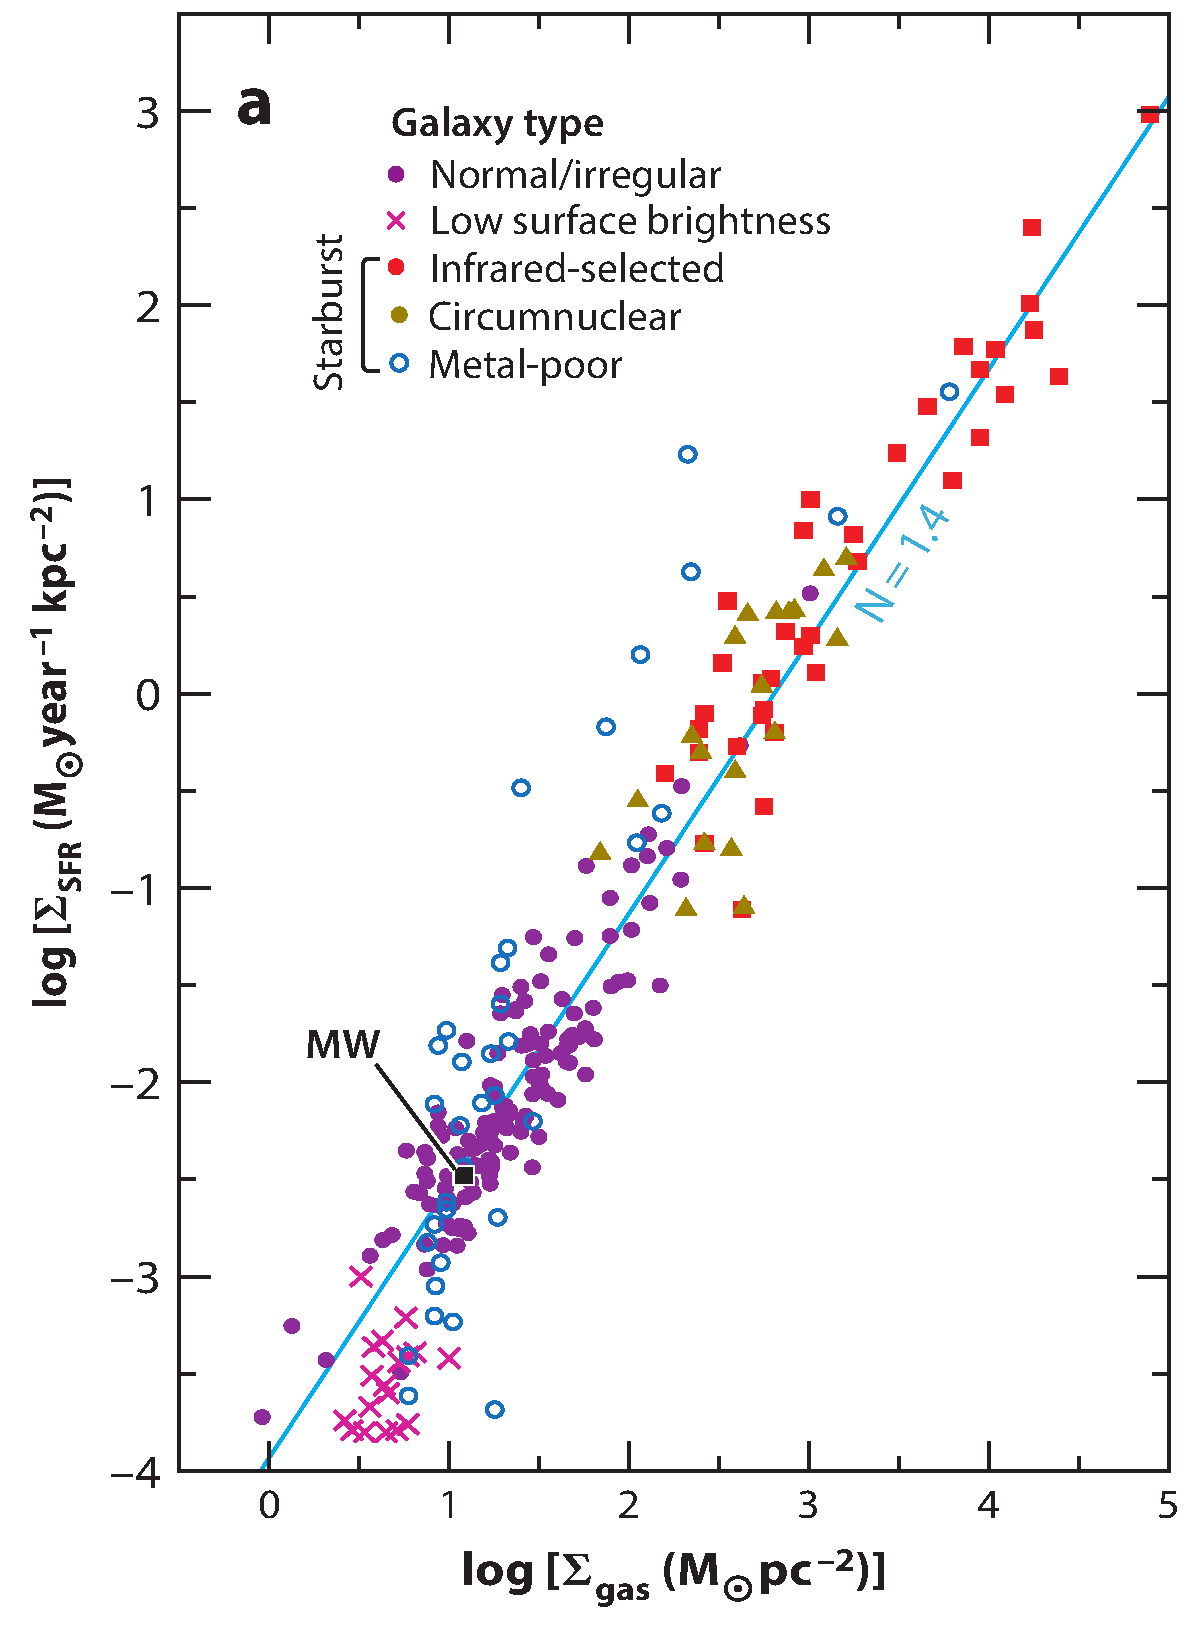
\includegraphics[width=0.4\textwidth]{KSlaw.pdf}
%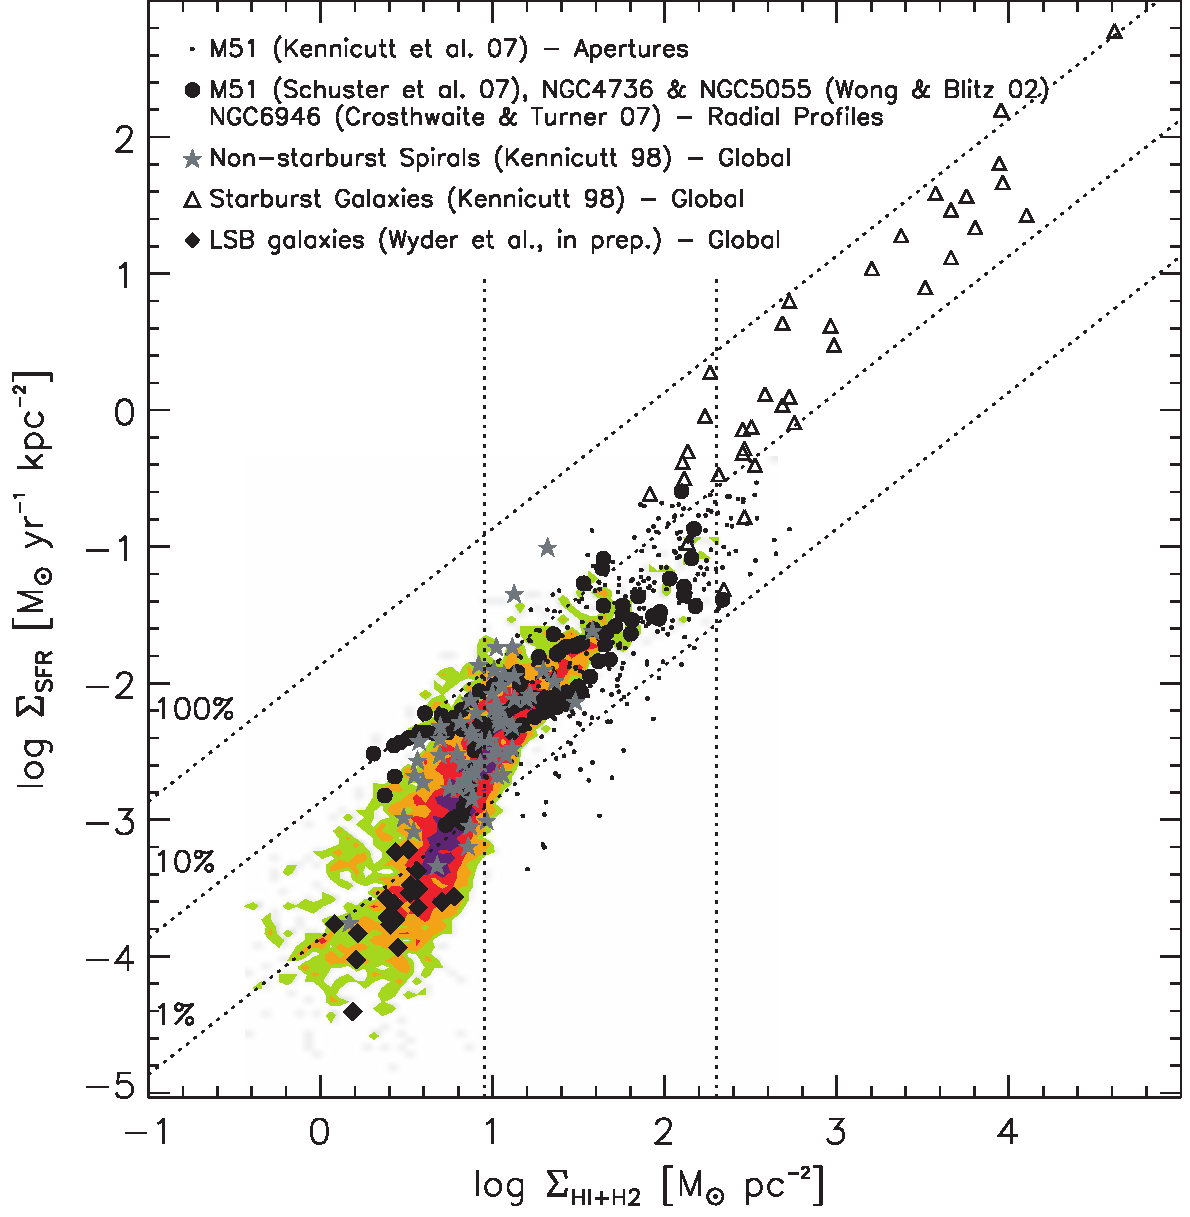
\includegraphics[width=0.52\textwidth]{bigiel08.pdf}
%\caption{Surface densities of SFR and total gas in nearby normal spiral
%        galaxies, low surface brightness galaxies, and star
%        bursts\citep[i.e.,][]{Bigiel2008}.  }
%\label{bigiel08}
%\end{figure}



\begin{landscape}
\begin{table}
\caption{ Observed quantities in the central positions} 
\label{tab:stack}
\centering
\scriptsize
\begin{tabular}{l l l l l l l l l l l l l l l l l l }
\hline
\toprule
Molecule &  \multicolumn{8}{c}{HCN} & \multicolumn{8}{c}{HCO+}\\
\midrule
Source     & W       & Err     & Wfree   & Err     & linewidth & GaussW  & Err     & linewidth$_g$ & W       & Err     & Wfree   & Err     & linewidth & GaussW  & Err     & linewidth$_g$ \\
           & (Kkm/s) & (Kkm/s) & (Kkm/s) & (Kkm/s) & (km/s)    & (Kkm/s) & (Kkm/s) & km/s          & (Kkm/s) & (Kkm/s) & (Kkm/s) & (Kkm/s) & (km/s)    & (Kkm/s) & (Kkm/s) & km/s          \\
           &(1)      & (2)     & (3)     & (4)     & (5)       & (6)     & (7)     & (8)           & (9)     & (10)    & (11)    & (12)    & (13)      & (14)    & (15)    & (16)          \\ 
\hline
ARP299     & 1.94    & 0.11    & 1.95    & 0.10    & 196       & 2.05    & 0.09    & 295$\pm$14    & 2.15    & 0.08    & 2.13    & 0.12    & 172       & 2.25    & 0.13    & 324 $\pm$21   \\
NGC253     & 36.9    & 0.6     & 36.8    & 0.5     & 132       & 37.8    & 0.5     & 155$\pm$2     & 48.8    & 0.5     & 48.7    & 0.4     & 137       & 50.3    & 0.3     & 157 $\pm$ 1   \\
NGC600     & 1.35    & 0.26    & 1.32    & 0.1     & 233       & 1.41    & 0.14    & 333$\pm$34    & 2.39    & 0.15    & 2.40    & 0.12    & 302       & 2.60    & 0.17    & 365 $\pm$ 23  \\
NGC891     & 0.89    & 0.19    & 0.92    & 0.13    & -         & 0.78    & 0.15    & 145$\pm$35    & $<$1.16 & 0.39    & $<$0.56 & 0.19    & -         & -       & -       & -             \\
maffei2    & 2.00    & 0.24    & 1.97    & 0.14    & 95        & 2.10    & 0.13    & 122$\pm$8     & 2.78    & 0.22    & 2.81    & 0.20    & 95        & 2.91    & 0.20    & 140$\pm$10    \\
NGC1068    & 5.90    & 0.28    & 5.89    & 0.23    & 145       & 6.02    & 0.25    & 200$\pm$9     & 1.27    & 0.34    & 1.26    & 0.21    & 113       & 1.46    & 0.20    & 140$\pm$20    \\
NGC1097    & 0.53    & 0.26    & 0.55    & 0.09    & 60        & 0.54    & 0.1     & 170$\pm$30    & $<$0.45 & 0.14    & $<$0.43 & 0.14    & -         & -       & -       & -             \\
NGC1365    & 4.5     & 0.31    & 4.44    & 0.49    & -         & 4.3     & 0.5     & 195$\pm$22    & -       & -       & -       & -       & -         & -       & -       & -             \\
IC342      & 1.95    & 0.20    & 1.90    & 0.16    & 35        & 1.89    & 0.17    & 47$\pm$5      & 2.13    & 0.29    & 2.19    & 0.16    & 43        & 2.12    & 0.17    & 44$\pm$4.0    \\
NGC1808    & 1.99    & 0.19    & 2.02    & 0.16    & 96        & 2.04    & 0.16    & 190$\pm$17    & 2.09    & 0.18    & 2.11    & 0.17    & 111       & 2.16    & 0.18    & 194$\pm$17    \\
NGC2146    & 1.07    & 1.06    & 1.05    & 0.17    & -         & 1.08    & 0.18    & 205$\pm$ 35   & 1.58    & 0.23    & 1.51    & 0.15    & 131       & 1.61    & 0.16    & 192$\pm$20    \\
NGC2903    & $<$0.60 & 0.20    & $<$0.3  & 0.10    & -         & -       & -       & -             & 0.52    & 0.10    & 0.53    & 0.08    & 166       & 0.55    & 0.09    & 126$\pm$24    \\
M82        & 5.89    & 0.33    & 5.83    & 0.36    & 109       & 6.02    & 0.41    & 181$\pm$13    & 17.50   & 0.51    & 17.5    & 0.50    & 143       & 17.97   & 0.57    & 184$\pm$9     \\
NGC3079    & 4.95    & 0.23    & 4.92    & 0.32    & 117       & 5.28    & 0.31    & 204$\pm$12    & $<$1.9  & 0.64    & $<$1.8  & 0.61    & -         & -       & -       & -             \\
NGC3521    & $<$0.60 & 0.20    & $<$0.32 & 0.10    & -         & -       & -       & -             & $<$2.4  & 0.8     & 0.64    & 0.15    & -         & 0.66    & 0.14    & 180$\pm$47    \\
NGC3627    & 1.37    & 0.33    & 1.30    & 0.20    & 77.6      & 1.31    & 0.20    & 140$\pm$23    & 0.60    & 0.21    & 0.64    & 0.16    & -         & 0.67    & 0.17    & 156$\pm$39    \\
NGC3628    & 3.02    & 0.16    & 3.02    & 0.16    & 135       & 3.27    & 0.16    & 185$\pm$9     & 2.83    & 0.22    & 2.84    & 0.22    & 133.6     & 2.87    & 0.25    & 182$\pm$17    \\
NGC4631    & $<$0.80 & 0.26    & $<$0.48 & 0.16    & -         & -       & -       & -             & $<$0.93 & 0.31    & $<$0.37 & 0.13    & -         & -       & -       & -             \\
NGC4736    & 0.40    & 0.09    & 0.40    & 0.08    & -         & 0.39    & 0.09    & 151$\pm$40    & $<$0.33 & 0.11    & $<$0.33 & 0.11    & -         & -       & -       & -             \\
M83        & 1.54    & 0.39    & 1.50    & 0.27    & -         & 1.72    & 0.34    & 167$\pm$35    & 1.09    & 0.32    & 1.02    & 0.24    & -         & 1.02    & 0.24    & 49$\pm$11     \\
NGC5457    & 0.84    & 0.11    & 0.83    & 0.07    & 180       & 0.85    & 0.08    & 195$\pm$21    & $<$0.36 & 0.12    & $<$0.32 & 0.11    & -         & -       & -       & -             \\
NGC6946    & 1.34    & 0.29    & 1.47    & 0.26    & -         & 1.39    & 0.27    & 98$\pm$19     & 1.89    & 0.28    & 1.73    & 0.25    & 59        & 2.05    & 0.30    & 143$\pm$10    \\
\hline
\end{tabular}
\end{table}
\end{landscape}







\begin{figure}
\centering

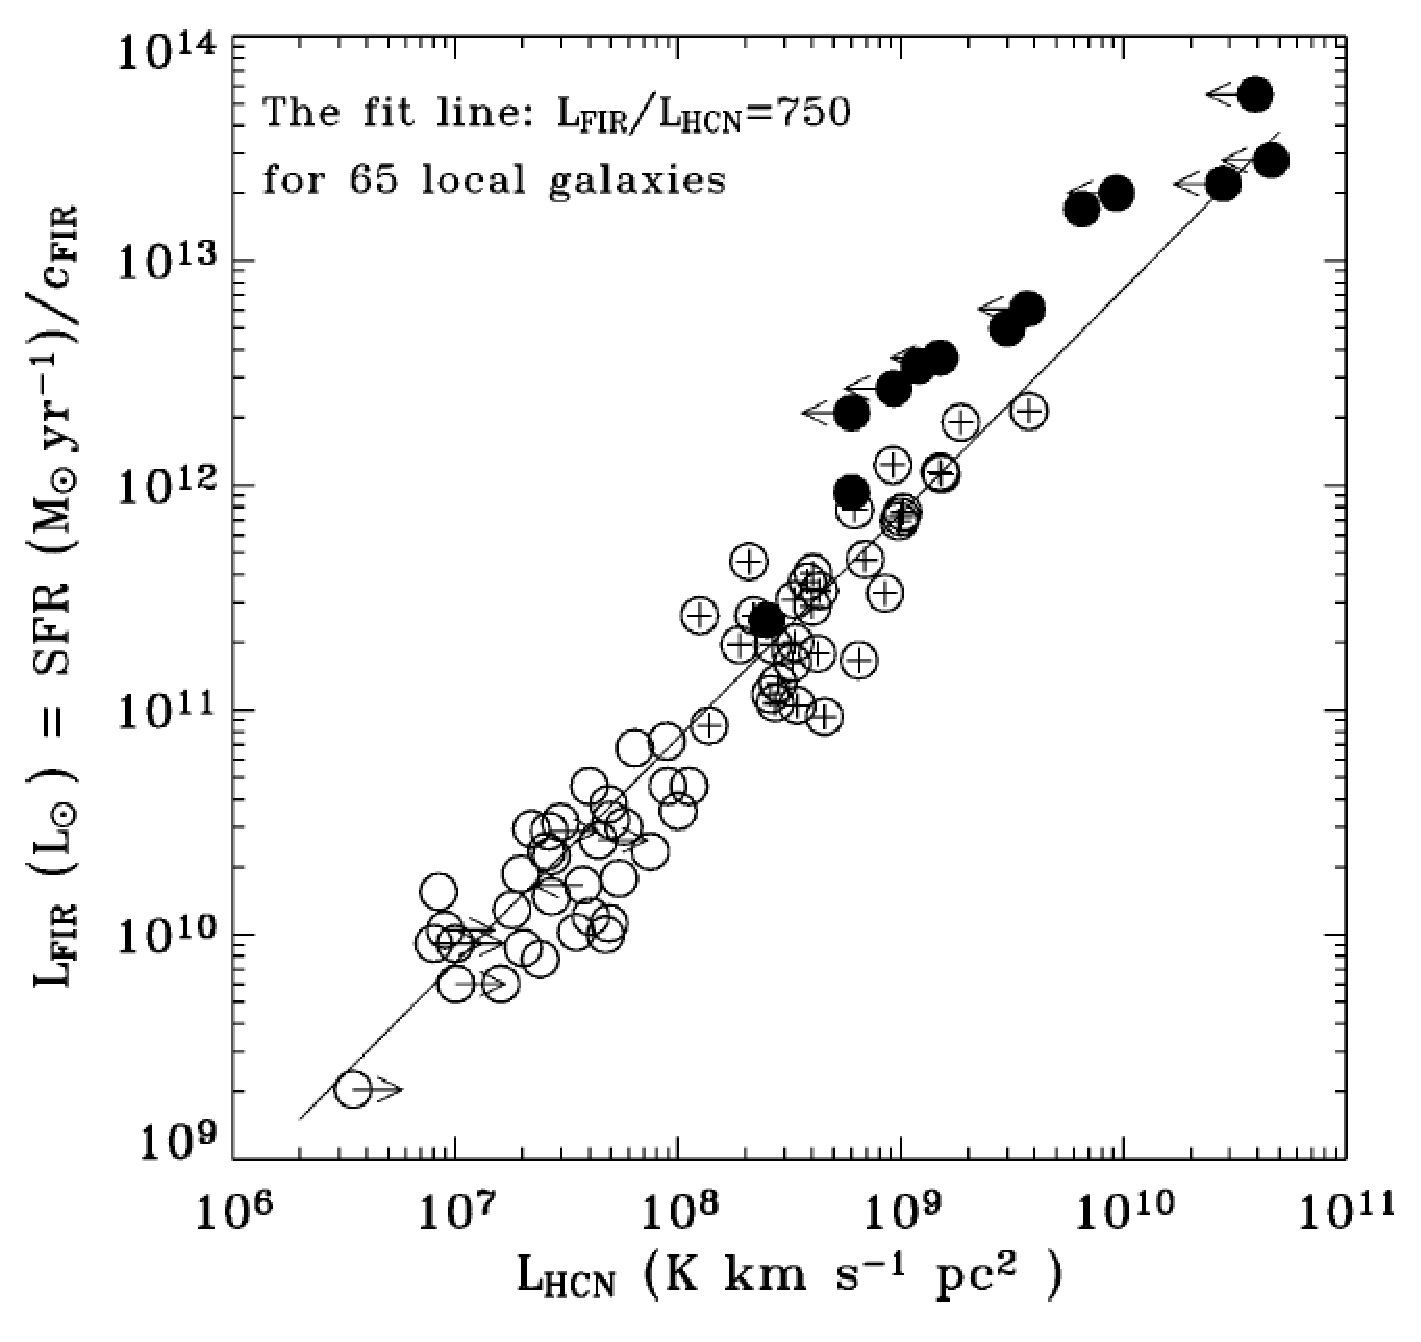
\includegraphics[width=0.3\textwidth]{Gao07.eps}
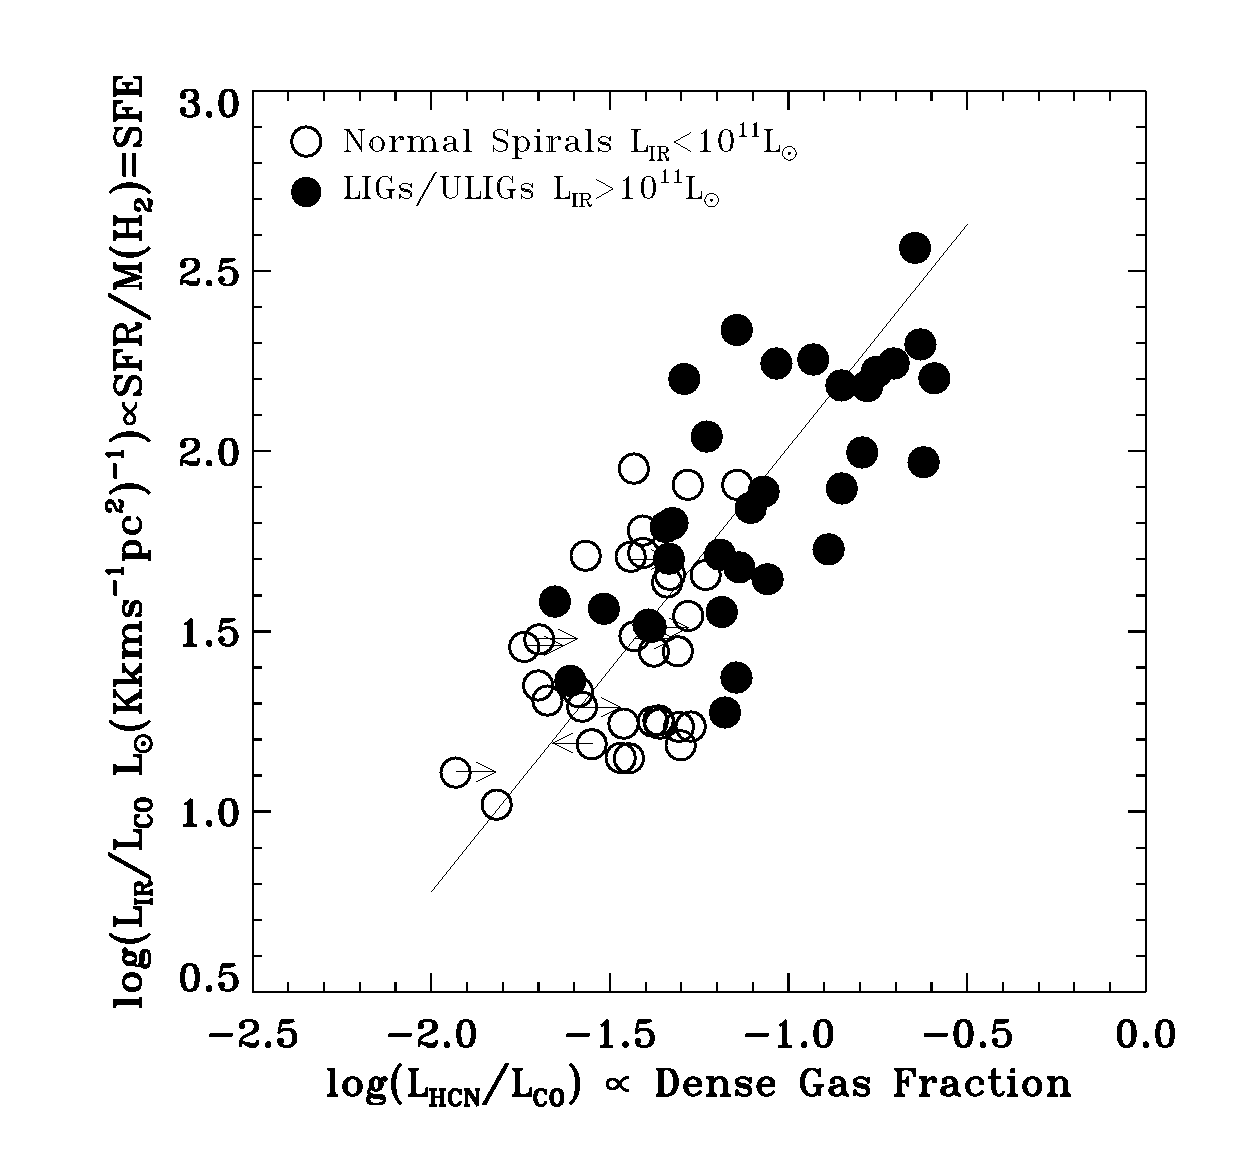
\includegraphics[width=0.32\textwidth]{gs04.eps}
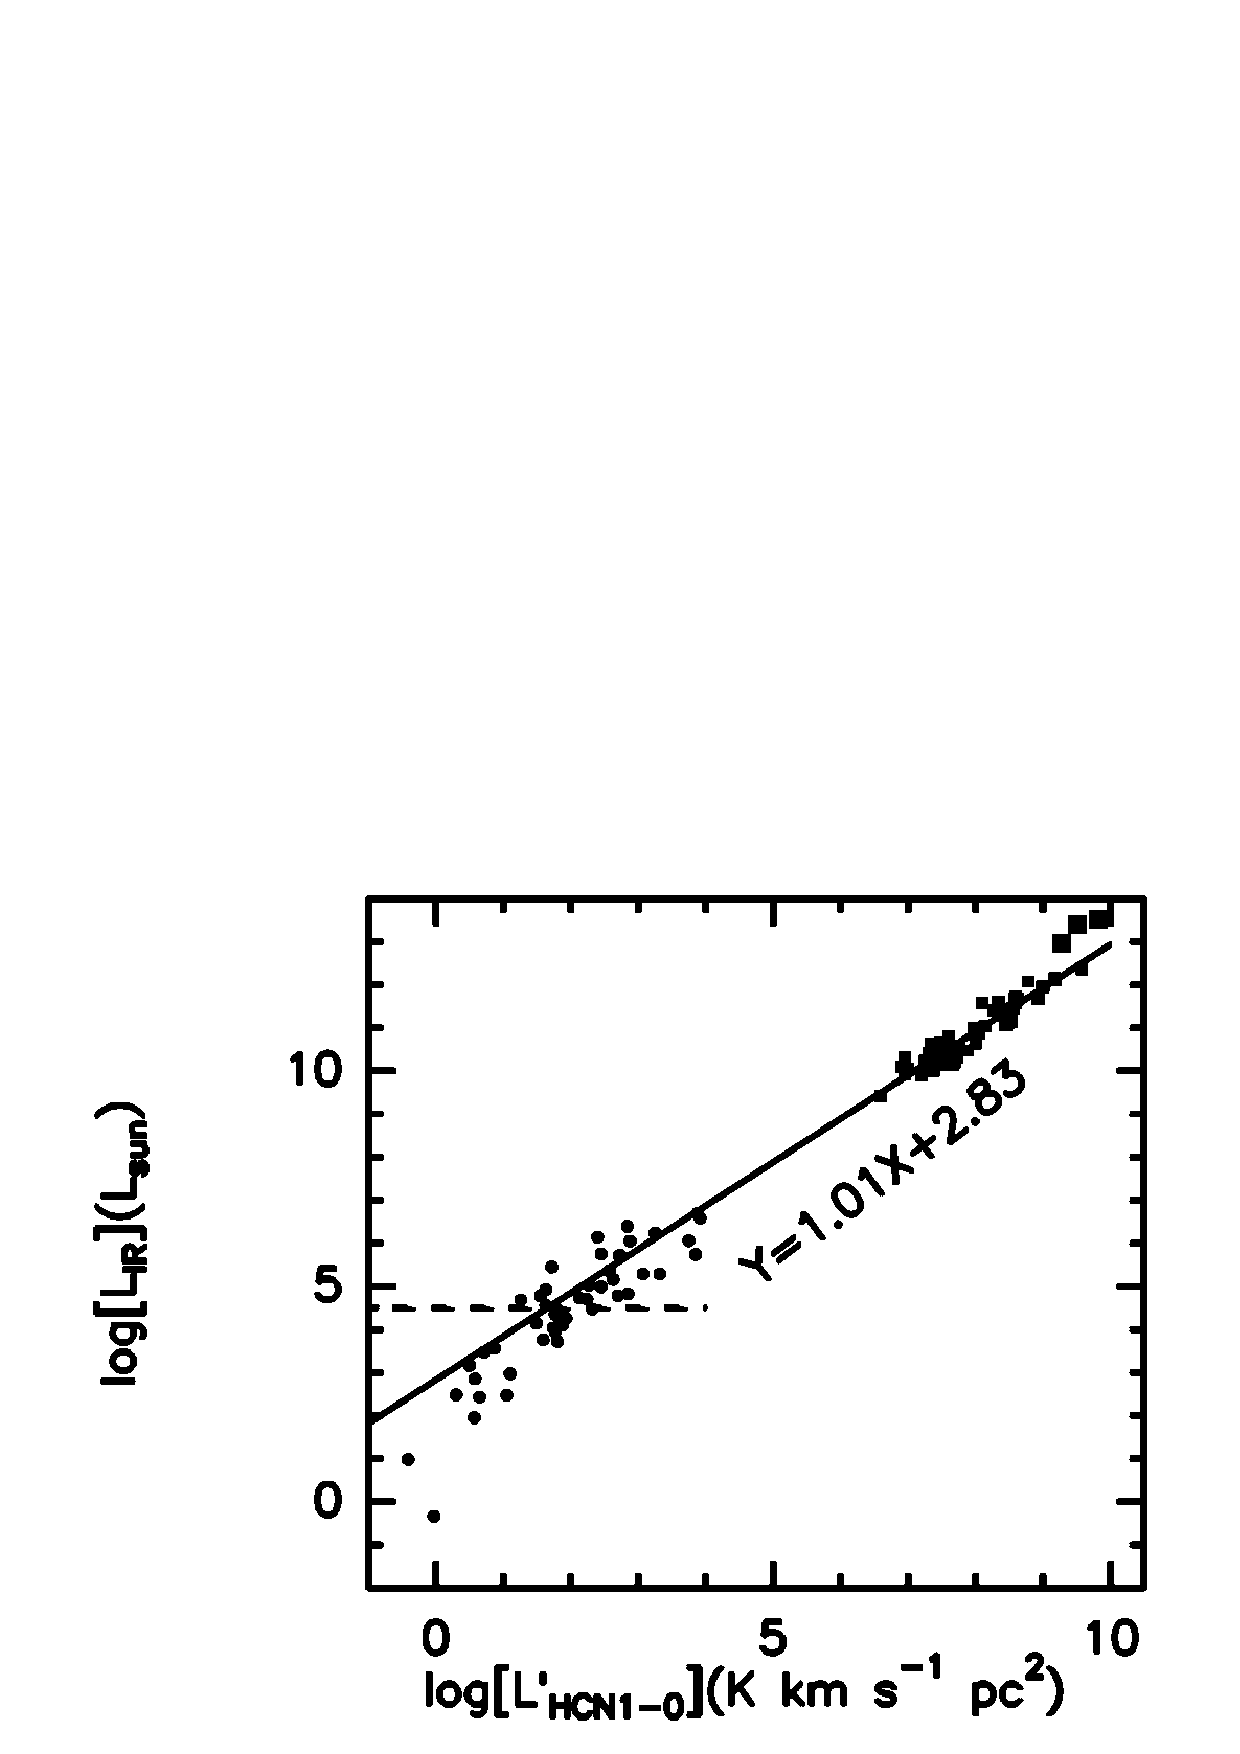
\includegraphics[width=0.35\textwidth]{wu05b.pdf}

\caption{Left: The HCN-FIR correlation (the fit is for local normal galaxies
        with a slope of 1 (open circles)).  Filled circles are high-$z$
        AGN/galaxies \citep{Gao2007} and circles with plus signs are local
        (U)LIRGs.  Middle: The correlation between $L_{\rm HCN}/L_{CO}$ and
        $L_{\rm IR}/L_{\rm CO}$ for a local sample \citep{gs04a}. Right: The
        correlation between $L_{\rm IR}$ and $L_{\rm HCN}$ for Galactic and
        extragalactic sources \citep{weg05}.}
\label{fig:hcn10}
\end{figure}

\begin{figure}
\centering
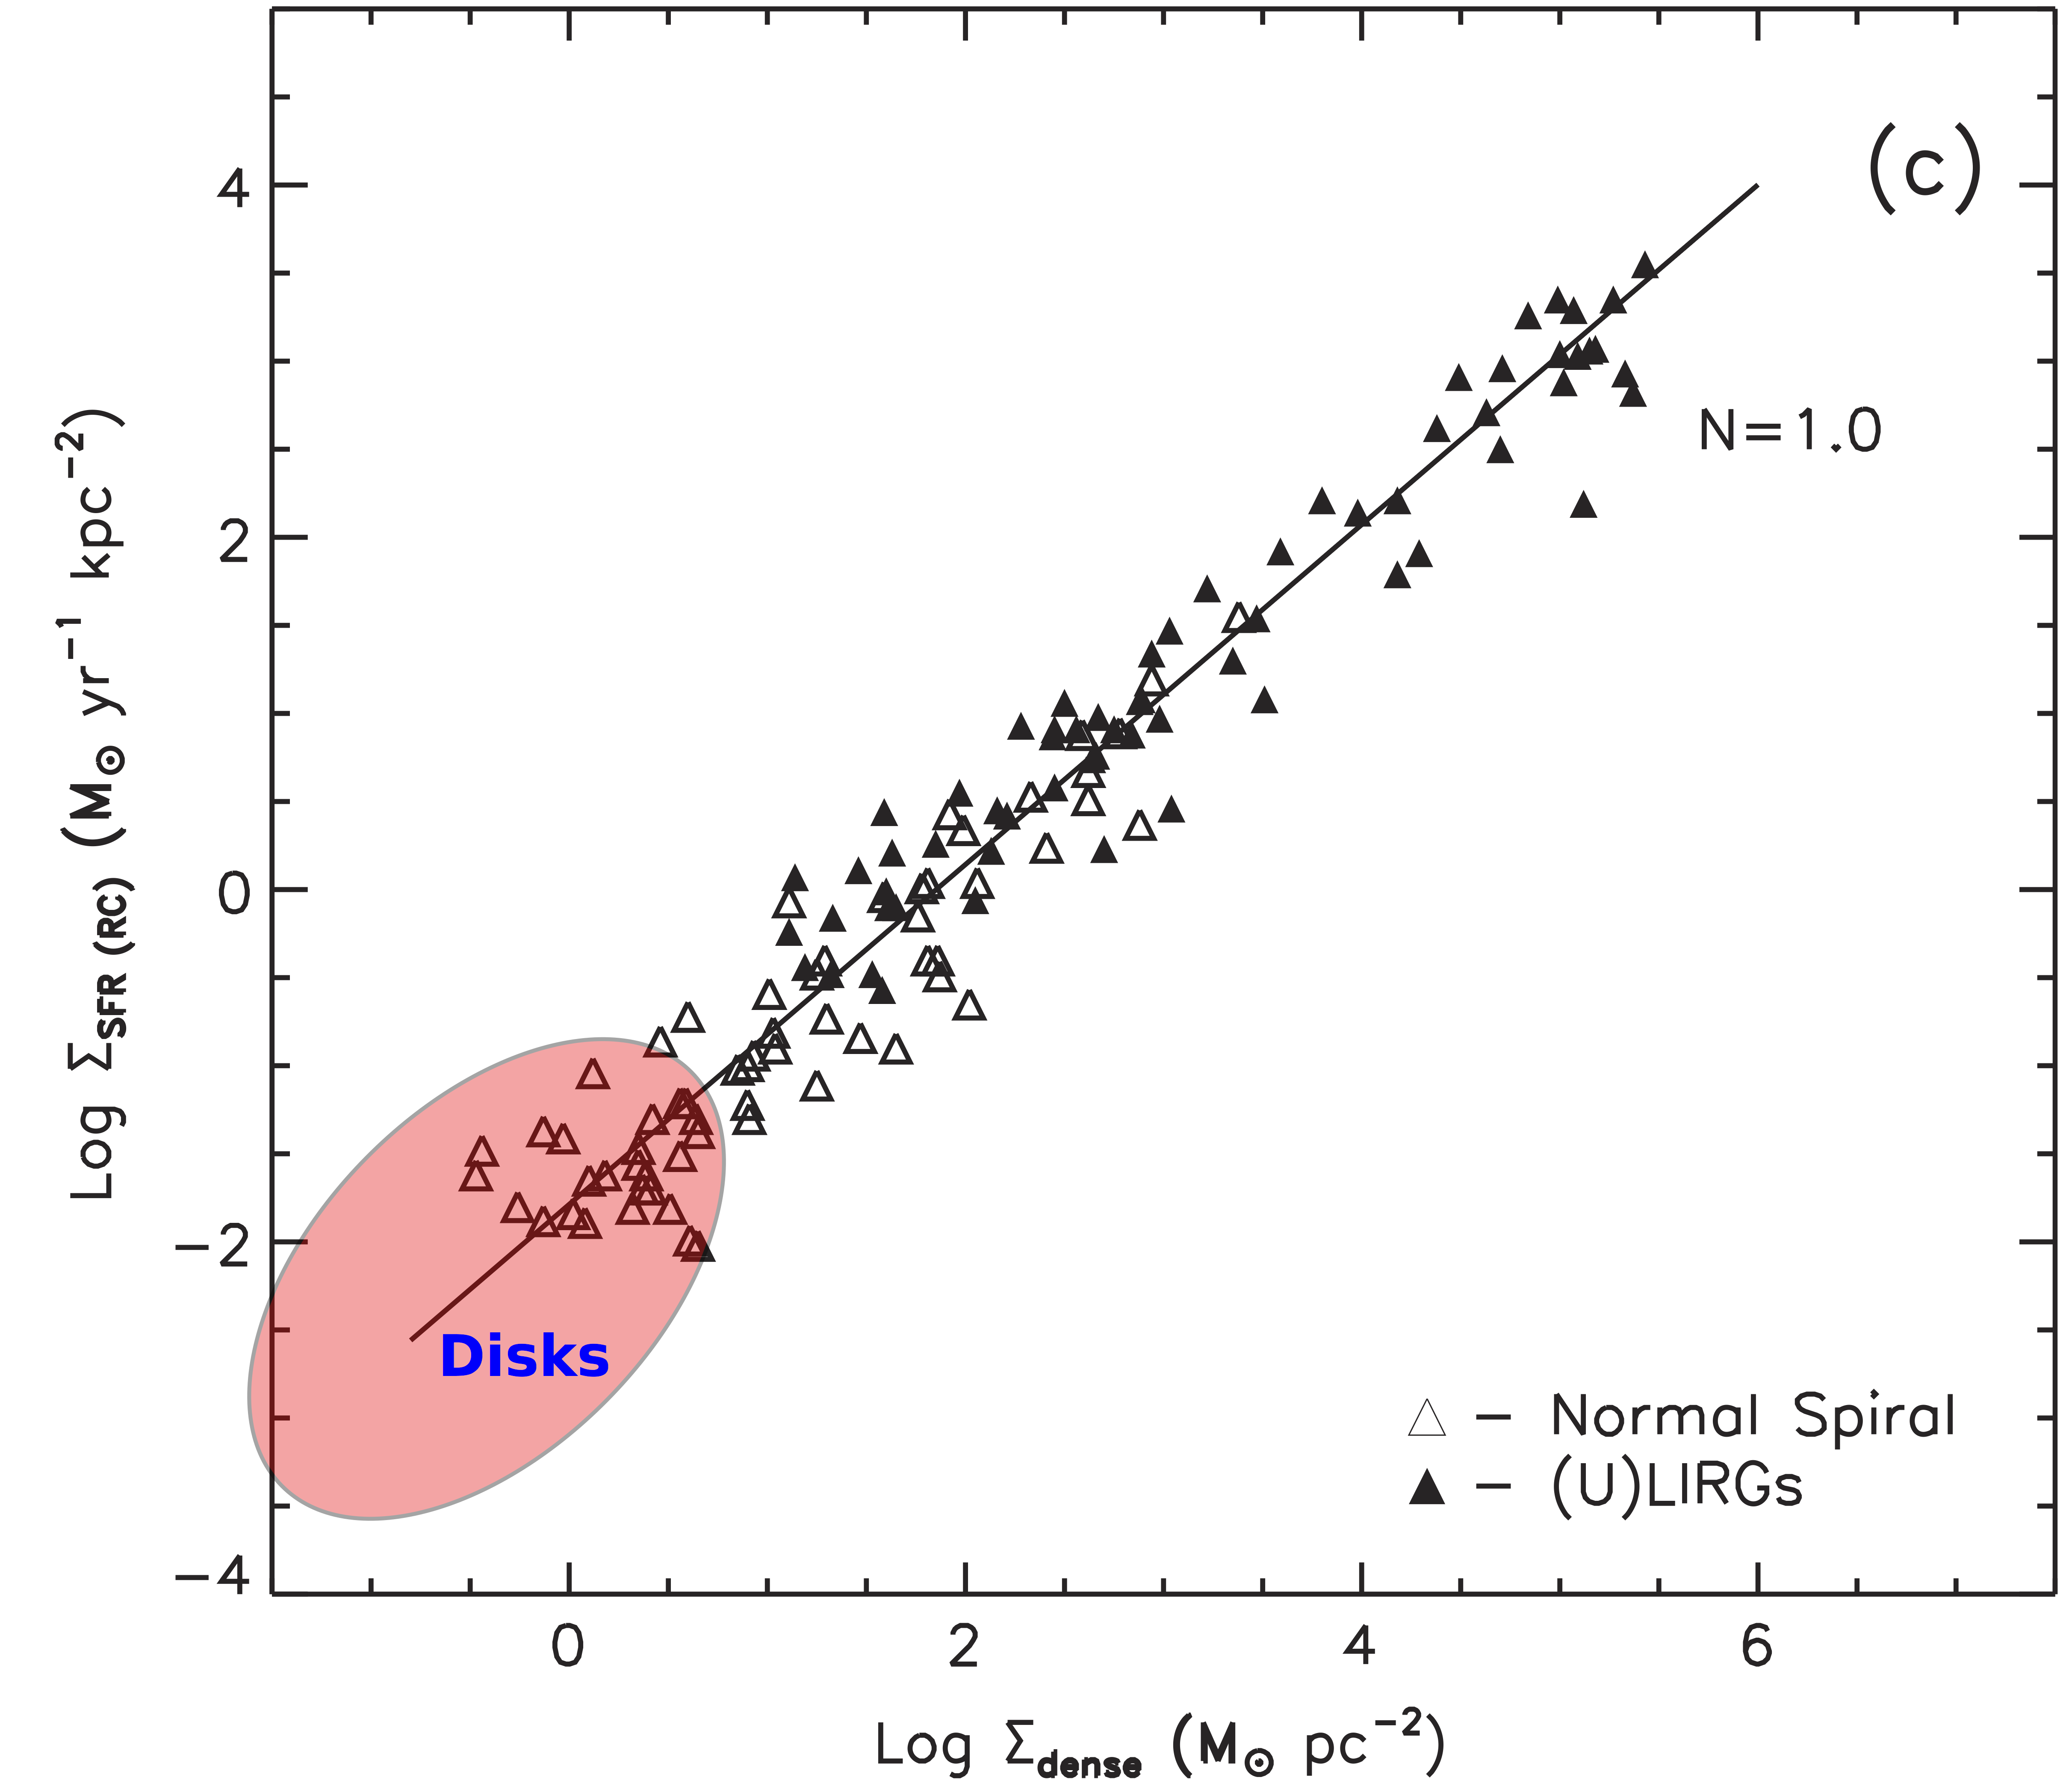
\includegraphics[width=0.6\textwidth]{HCN_IR.png}
\caption{
${\rm \Sigma_{dense}}$ as a function of $\Sigma_{\rm SFR}$. The ${\rm \Sigma_{dense}}$ 
        - $\Sigma_{\rm SFR}$ relation is the tightest one among all correlations, 
        and it is linear (N=$1.01 \pm 0.02$). Fitting to normal galaxies and (U)LIRGs separately 
yields identical linear correlation within the uncertainties.} 
\label{fig:hcn-ir}
\end{figure}






\begin{figure}
\centering

%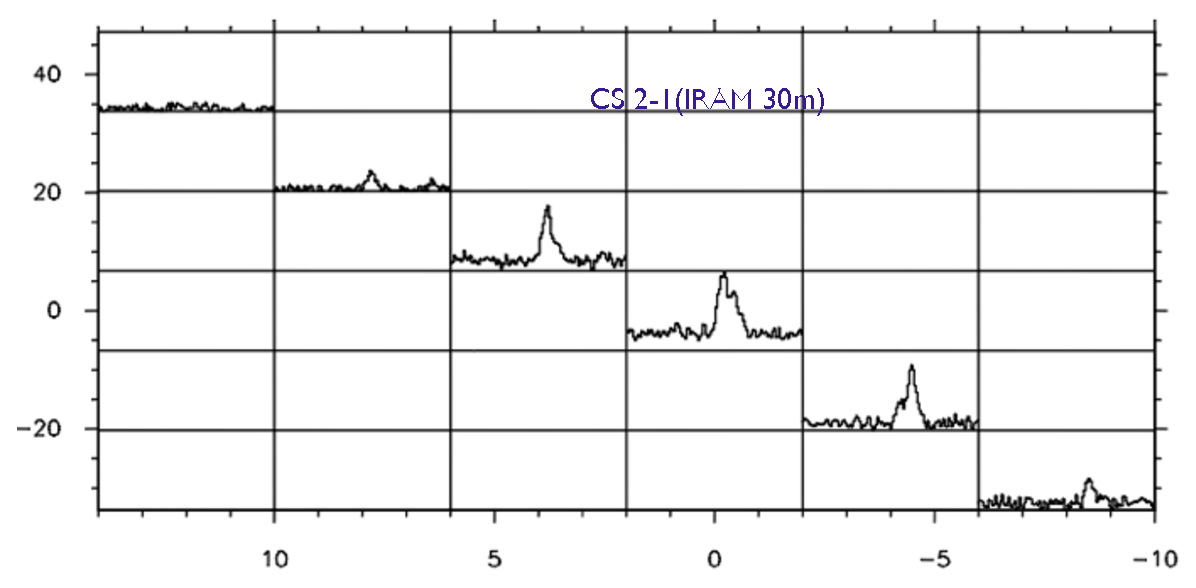
\includegraphics[width=0.8\textwidth]{maffei2-1.eps}
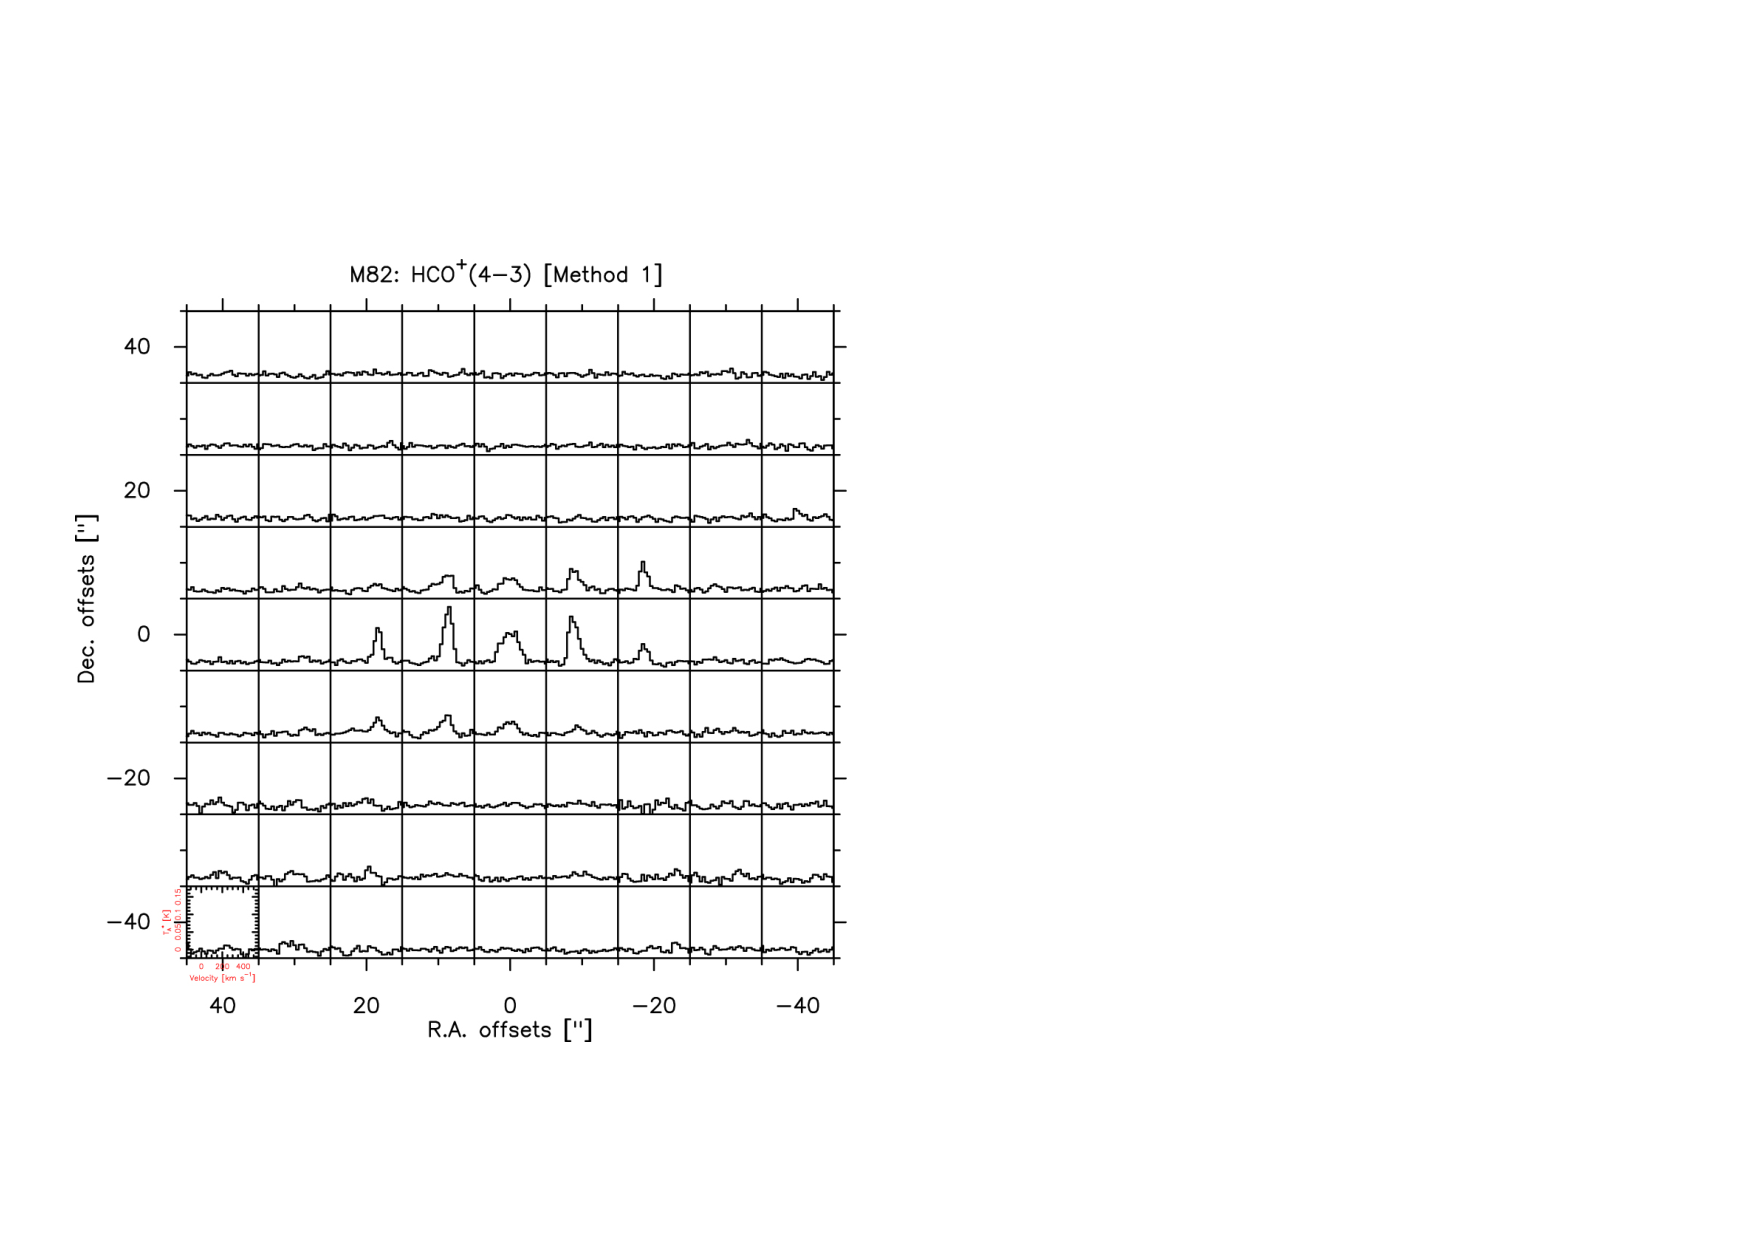
\includegraphics[width=0.49\textwidth]{Tan_M82.pdf}
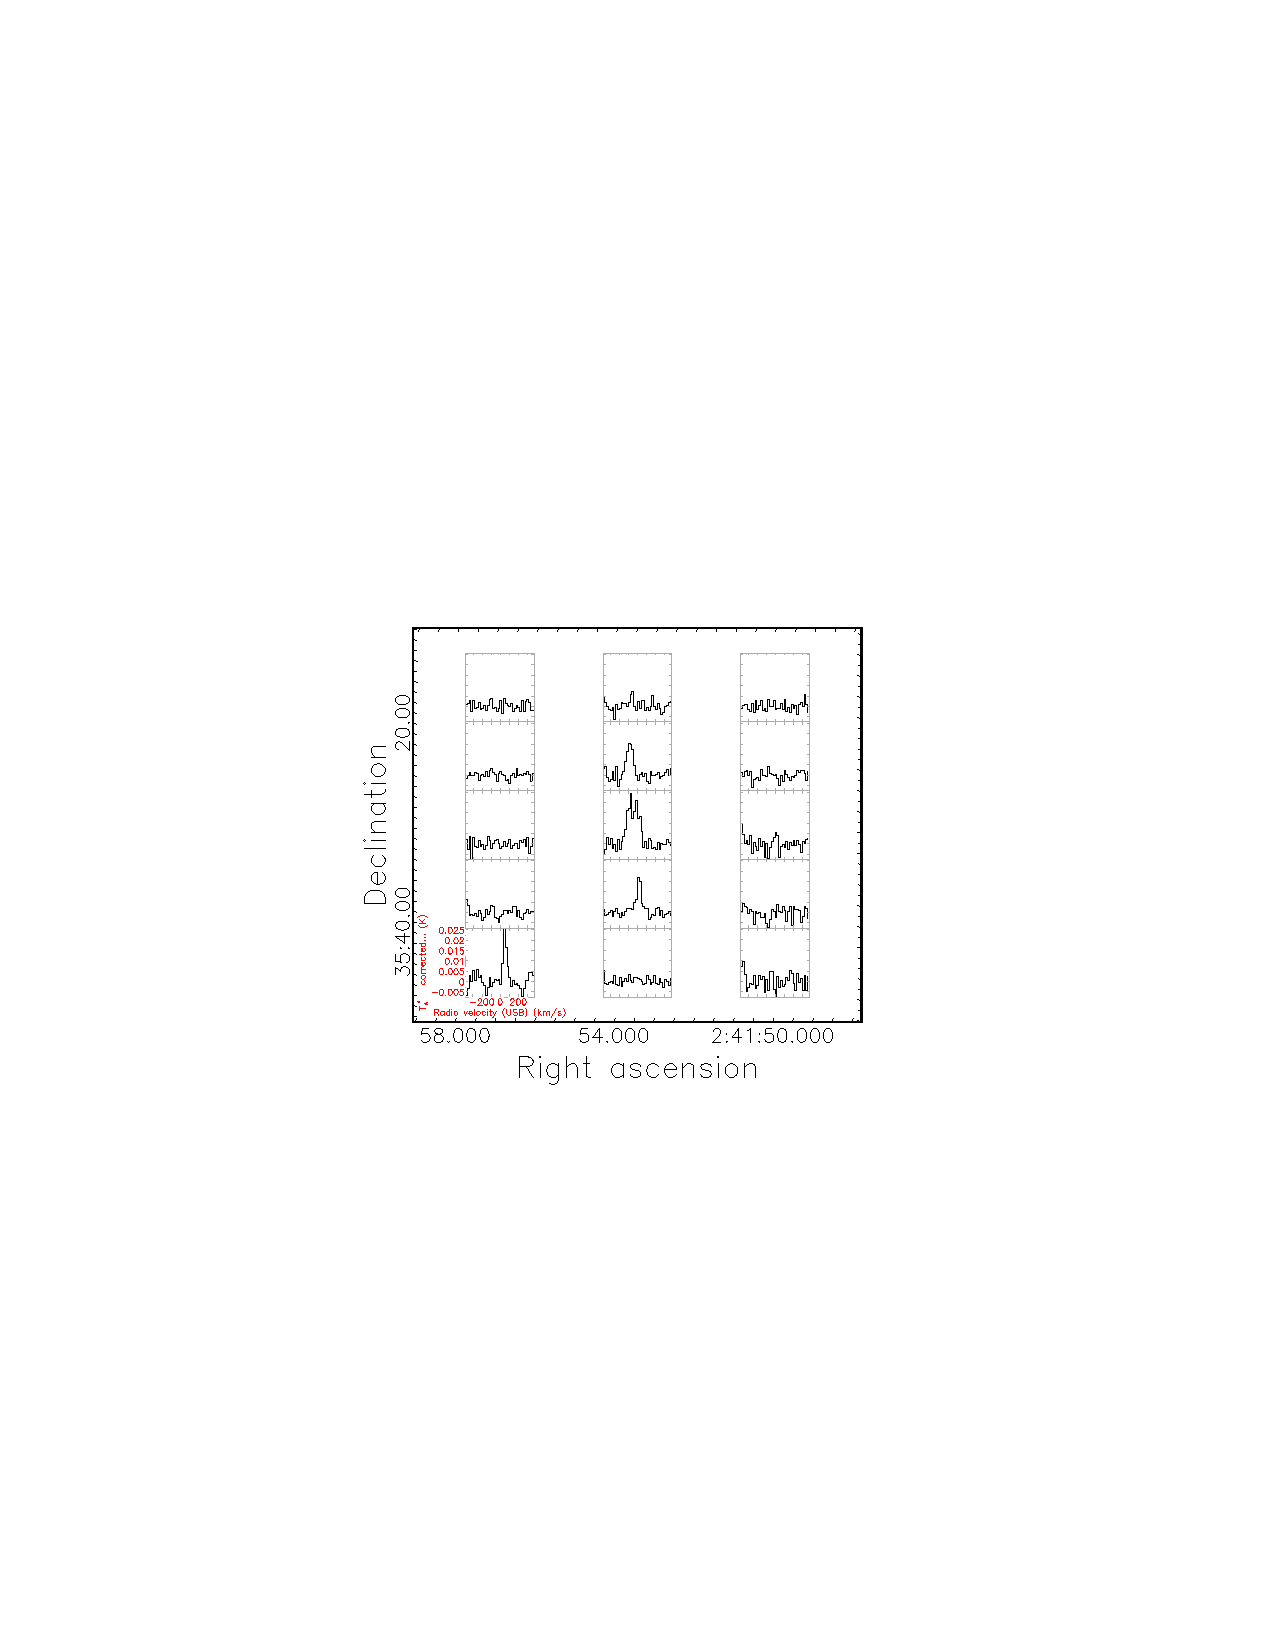
\includegraphics[width=0.49\textwidth]{maffei2-hco+.pdf}
\caption{
{\it left:} MALATANG \HCOP\ 4-3 spectra map in the central 90\arcsec $\times$ 90\arcsec region (grid spacing of 10\arcsec) of M82. All spectra are on the $T_A^*$ scale for the same range from −0.025 to 0.18 K and smoothed to 26 km\,s$^{−1}$ \citep{Tan:2018}. 
{\it right:} MALATANG \HCOP\ 4-3 spectra map of Maffei2, with a grid spacing of 15\arcsec.
}
\label{fig:maffei2}
\end{figure}






\begin{figure}
\centering
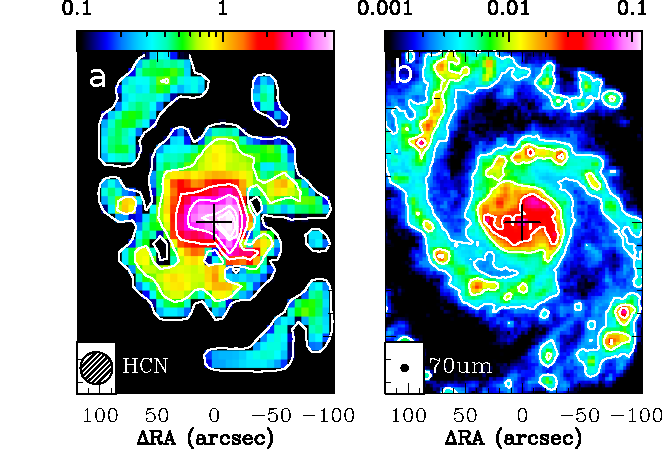
\includegraphics[width=0.8\textwidth]{M51_IR_HCN.pdf}

\caption{
(a) Integrated intensity map of \HCNoz\ of M~51. Contour levels are :        0.1, 0.6, 1.9, 3.4, 4.9, 5.4  \Kkms\ (on \Tmb\ scale) . (b) {\it Herschel} 70        \mum\ image with contour levels of 3, 9, 27,81 mJy/pixel.  The crosses        mark the central position of M~51 with $\alpha= 13:29:52.7$, $\delta=        47:11:43.0$ (J2000).} \label{fig:M51_IR_HCN}
\end{figure}

\begin{figure}
\centering
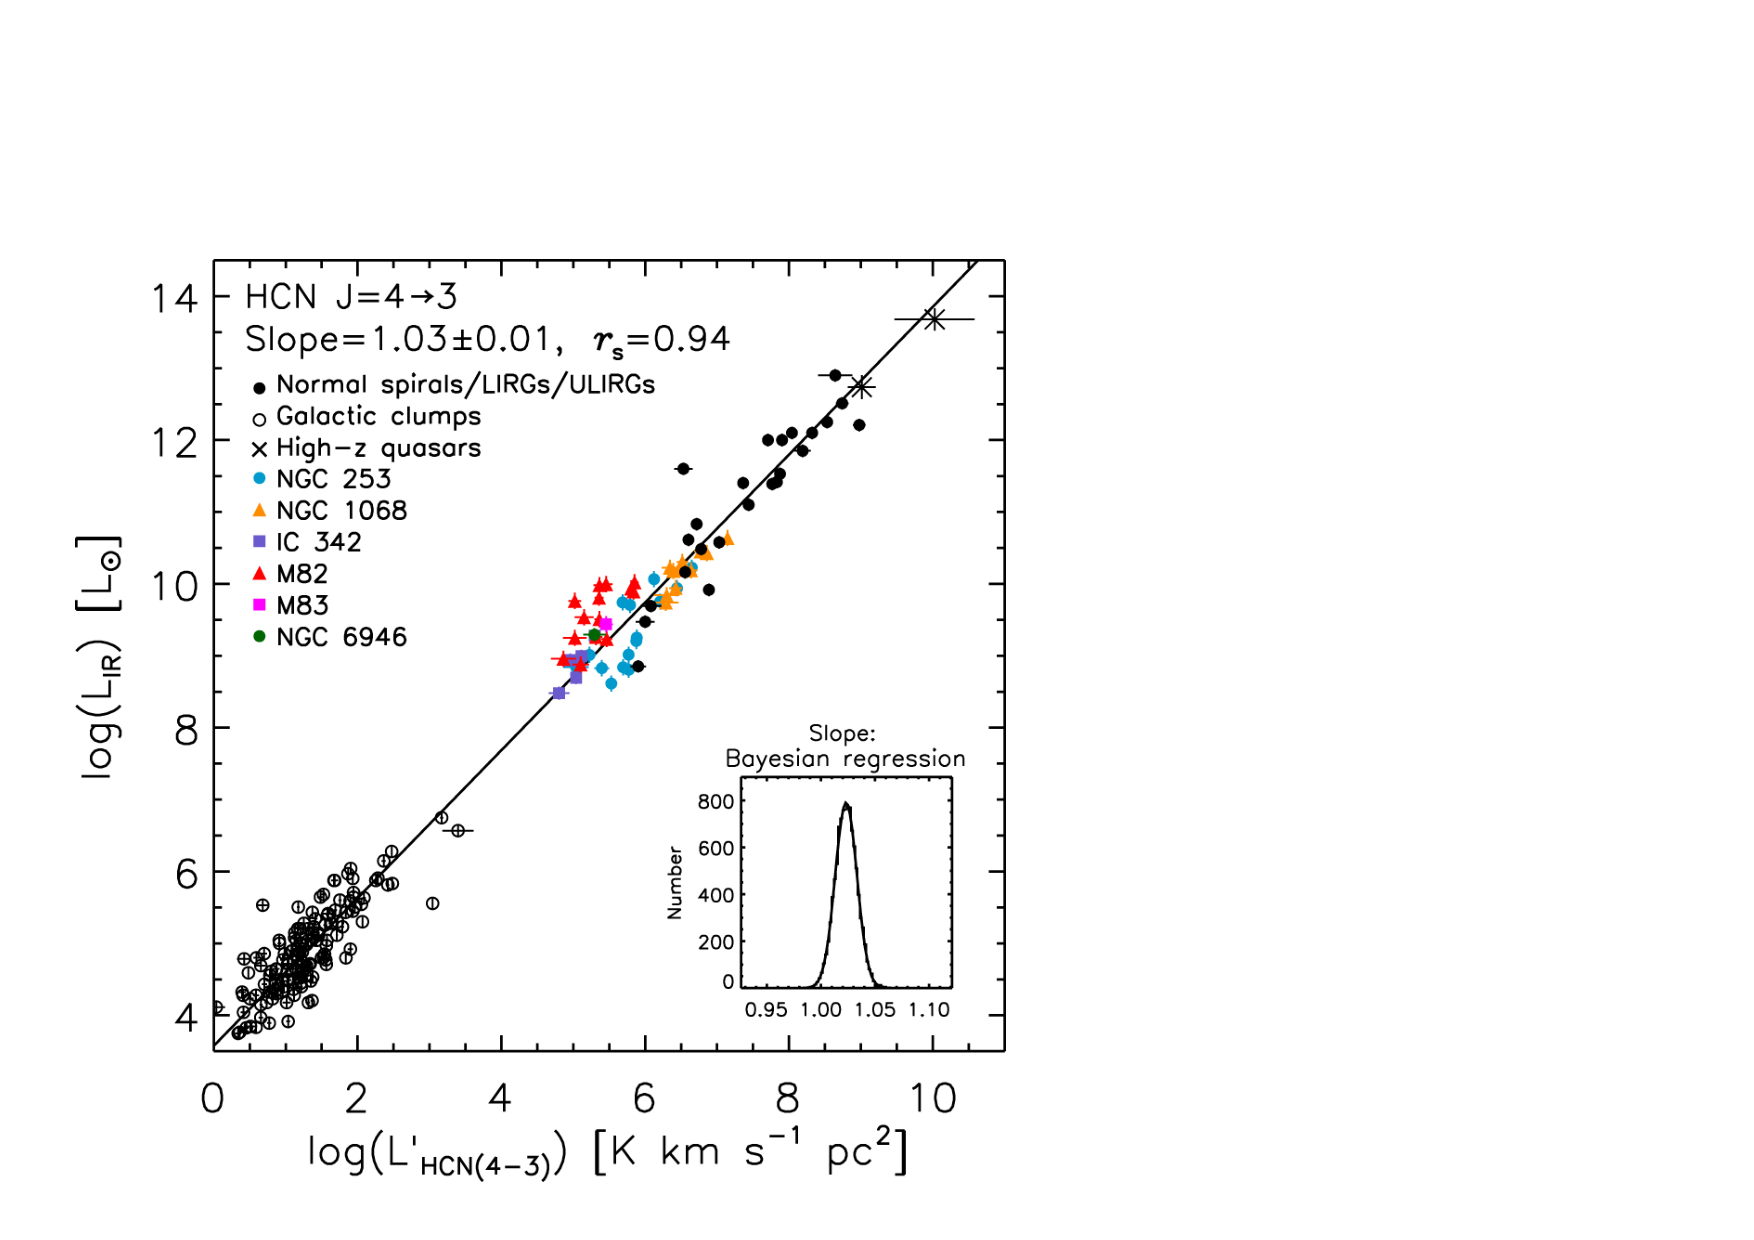
\includegraphics[width=0.6\textwidth]{Tan_relation.pdf}
%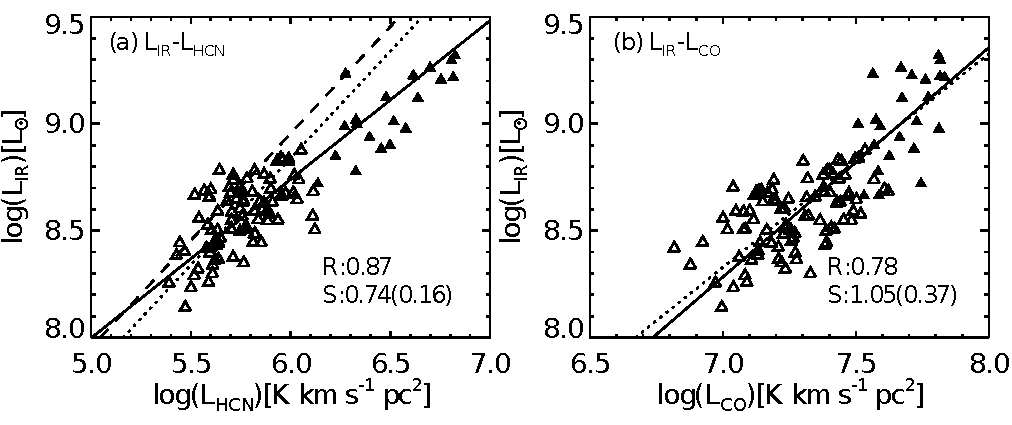
\includegraphics[width=0.8\textwidth]{M51.pdf}
\caption{
Correlation between HCN 4-3 and IR luminosities for Galactic
clumps (circles), MALATANG galaxies resolved at sub-kiloparsec scales (colored
symbols), normal galaxies and local (U)LIRGs (filled circles), and high-z quasars
(crosses). The upper limits of HCN 4-3 are not included in the fitting and
are not shown in this plot. The solid line represents the best-fit relation of
log \LIR=1.03($\pm$0.01)log $L'_{HCN 4–3}$+3.58. The probability density distribution
of the slope derived from the Bayesian fitting is shown in the inset panel. A
Spearman rank correlation analysis yields a correlation coefficient of 0.94  \citep{Tan:2018}.
%\LIR\ as a function of \LHCNoz in M~51.  Each symbol corresponds to an        individual pointing in the observations.  The pointings in the central        region are marked with filled triangles, and the open triangles show the        pointings on the disk.  The solid line shows the best fit for all data.        The dotted line indicates the fit with the data only on the disk.
} \label{fig:tan_relation}
\end{figure}




%%%
\begin{figure}
\centering
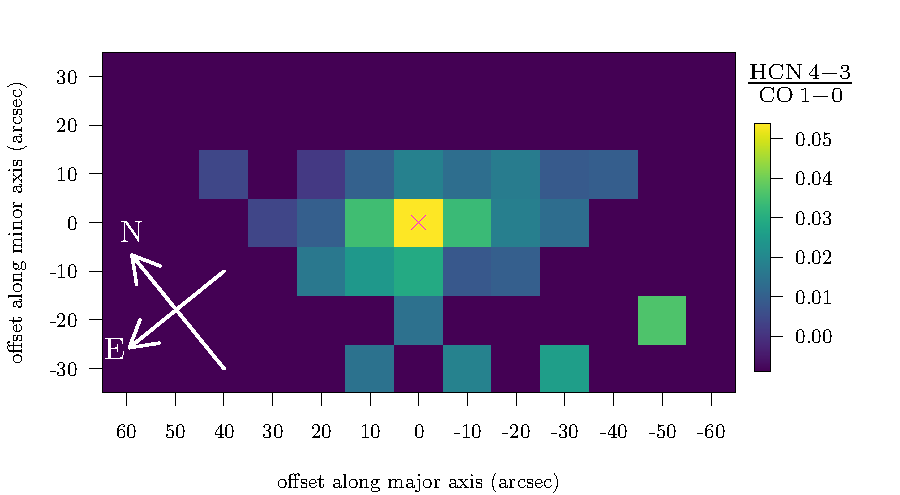
\includegraphics[width=0.48\textwidth]{Jiang_hcn_to_co10.pdf}
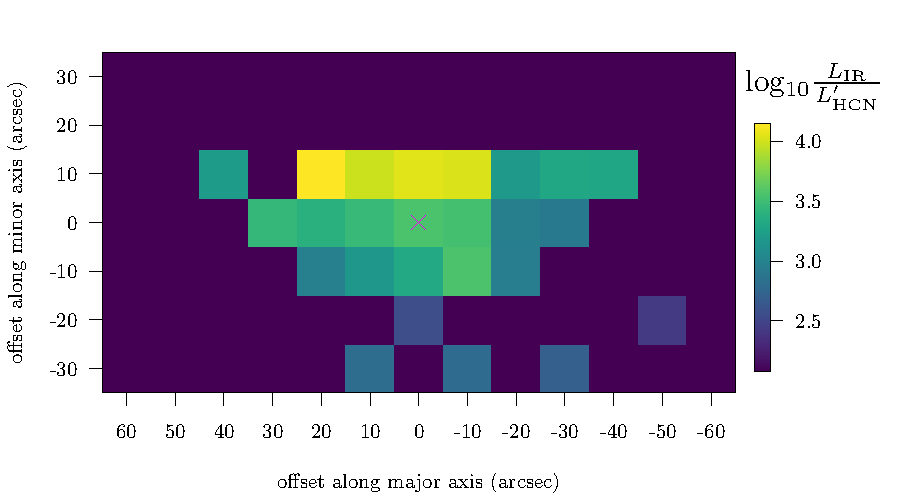
\includegraphics[width=0.48\textwidth]{Jiang_Lir_Lhcn.pdf}
%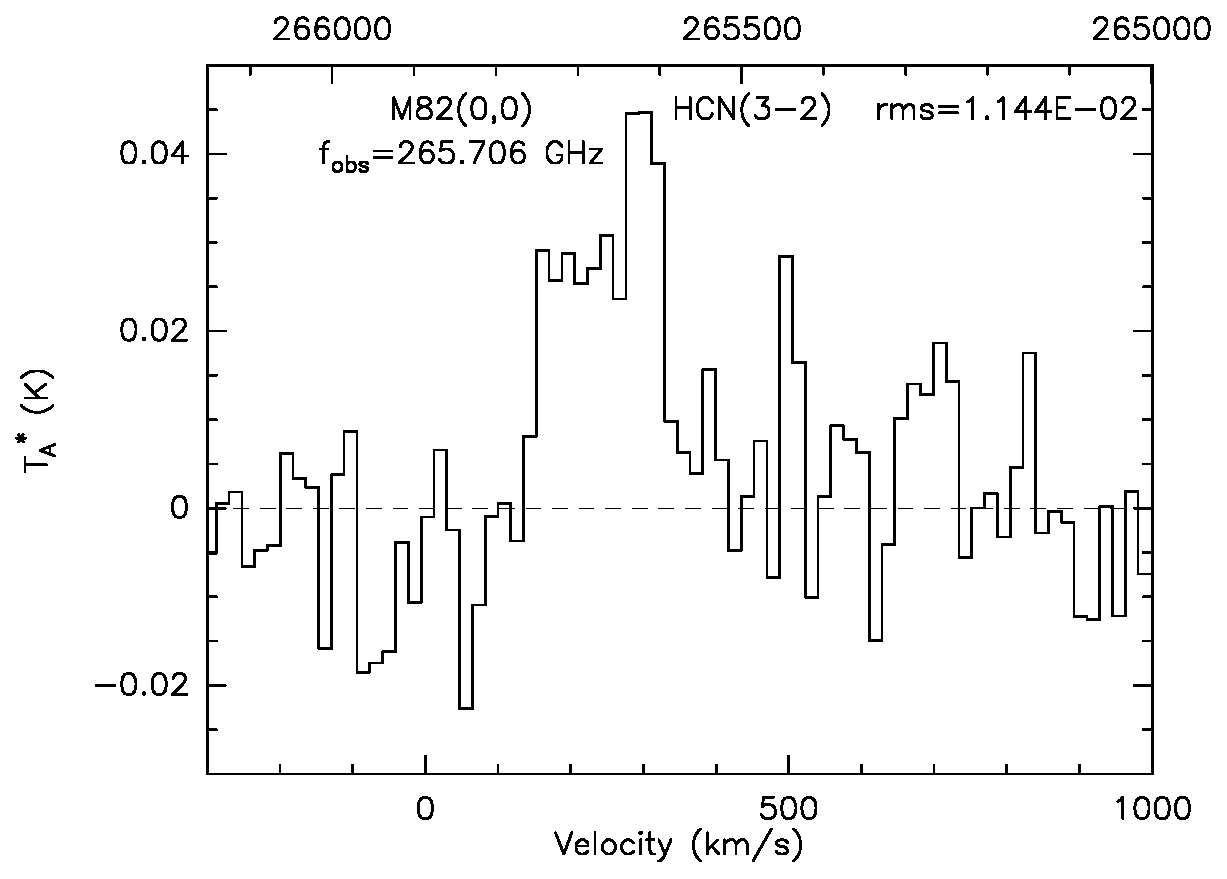
\includegraphics[width=0.43\textwidth]{m82_00.eps}
%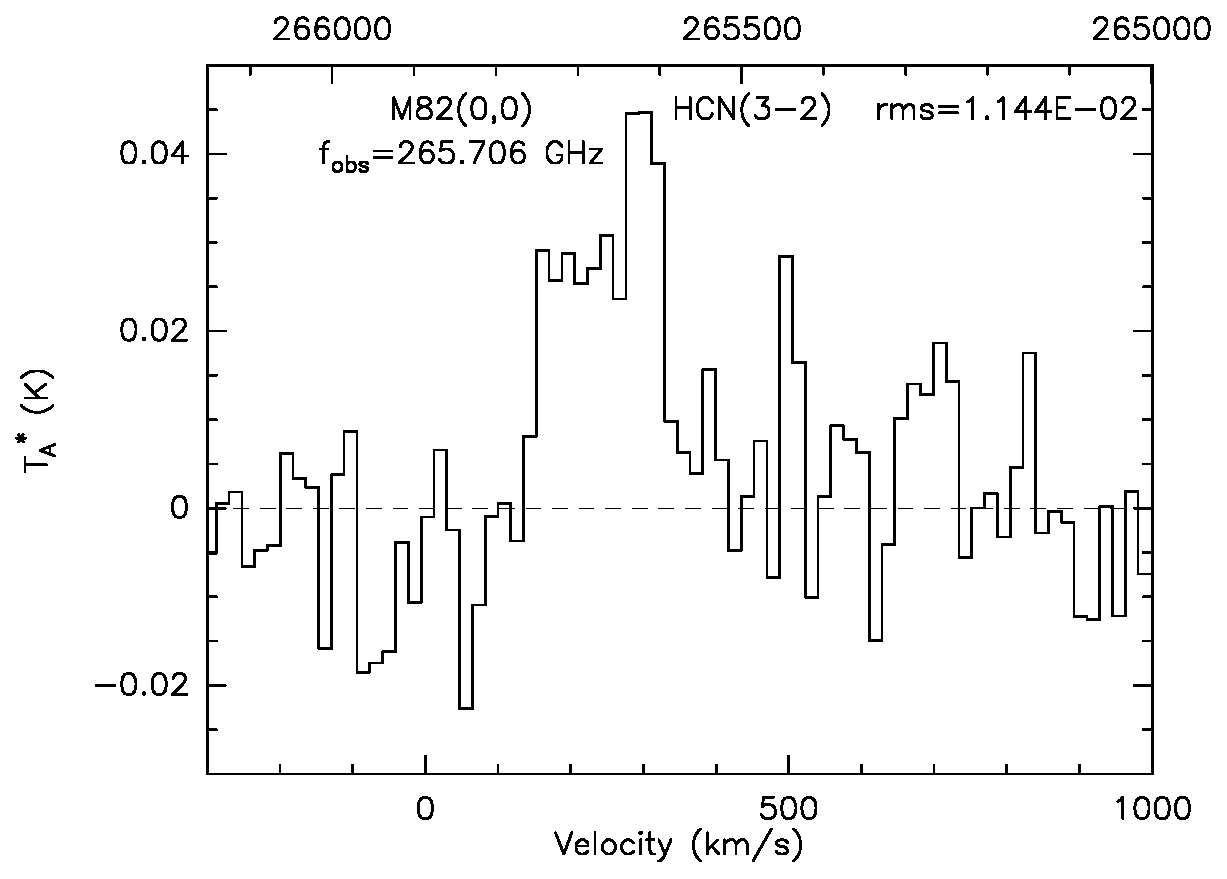
\includegraphics[width=0.43\textwidth]{m82_00.eps}
%\hskip10pt
%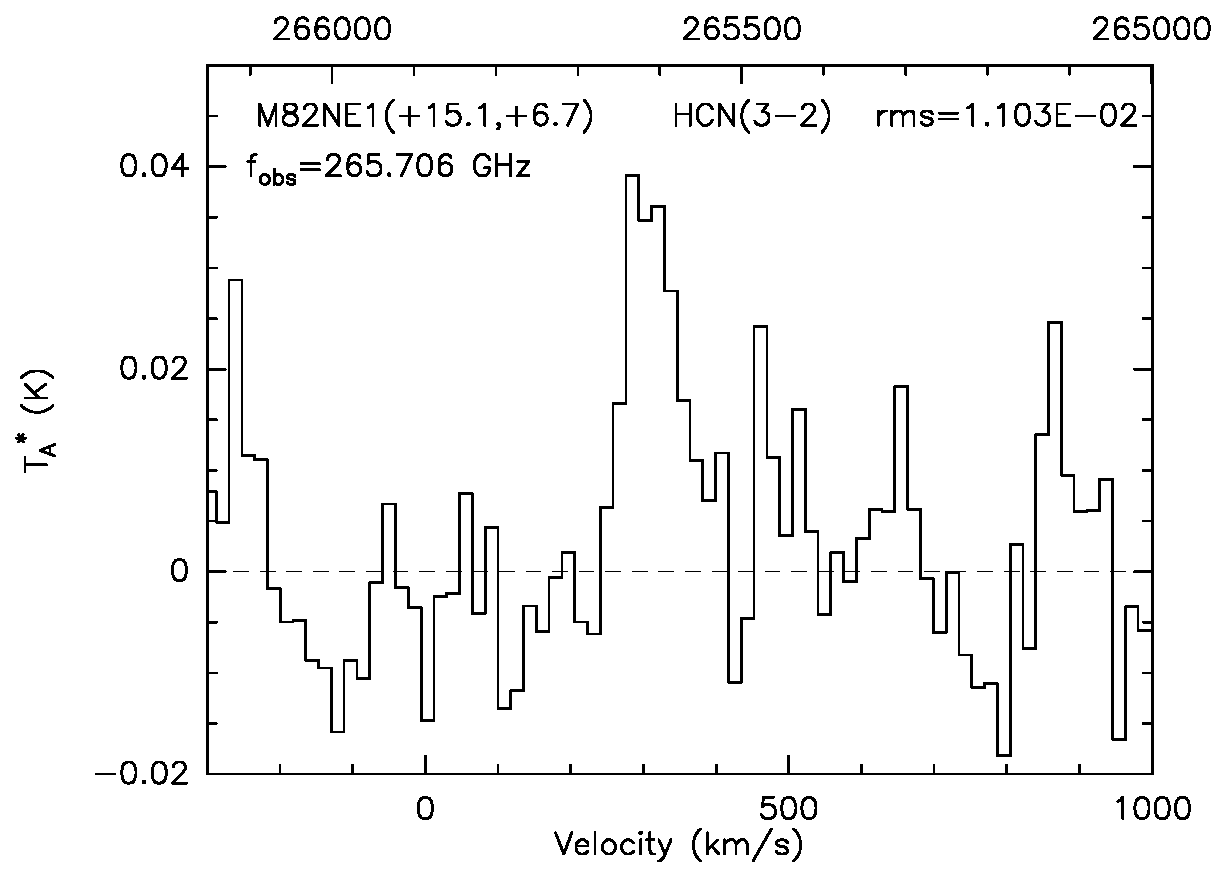
\includegraphics[width=0.43\textwidth]{m82_ne01.eps}
%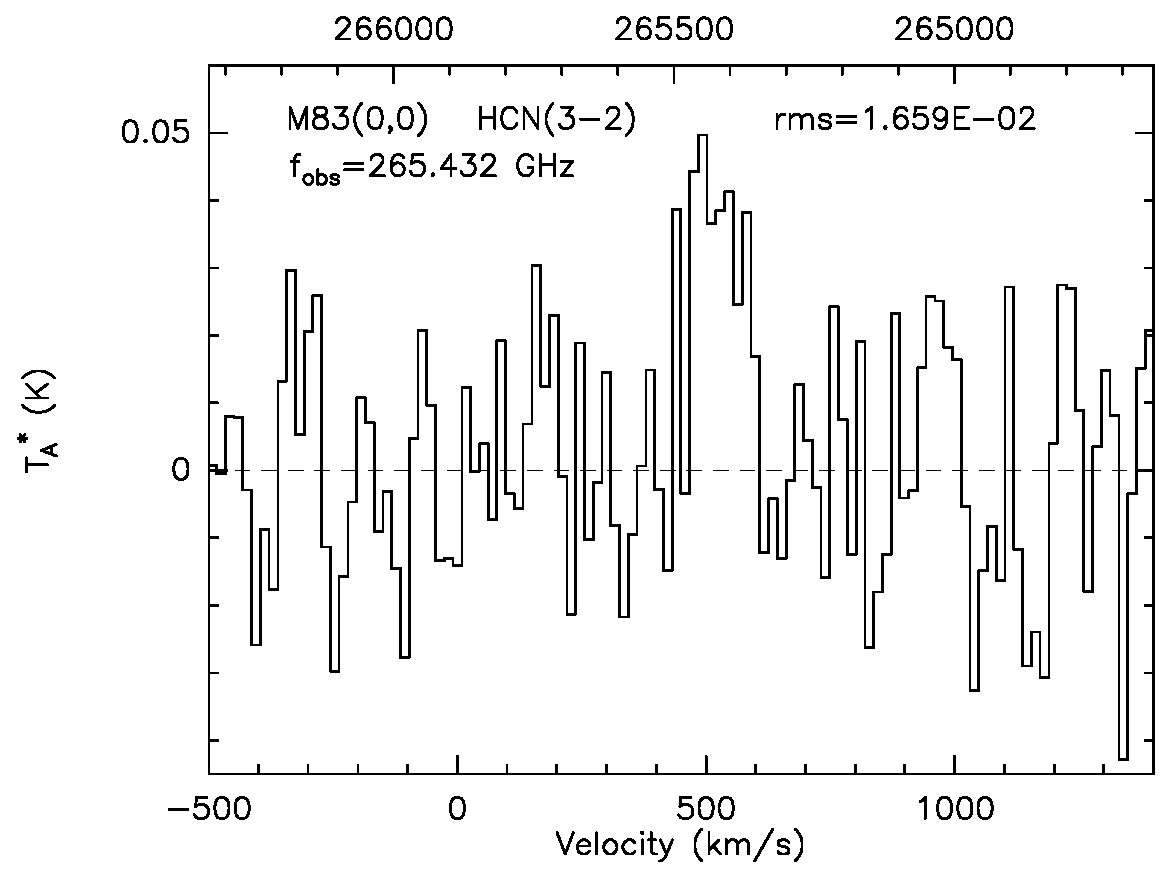
\includegraphics[width=0.43\textwidth]{m83_00.eps}
%\hskip10pt
%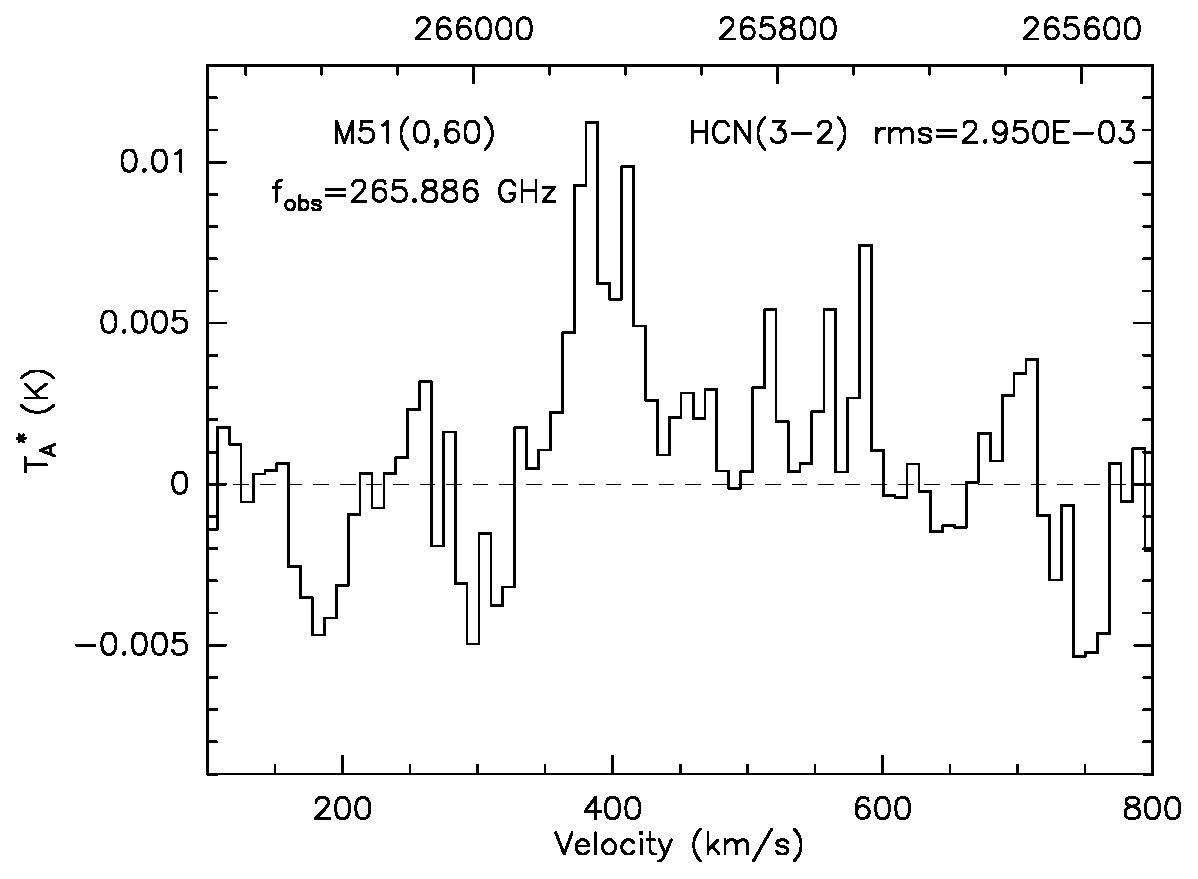
\includegraphics[width=0.43\textwidth]{m51_00.eps}
\caption{
{\it Left:} ratio map of HCN 4-3/CO 1-0 with MALATANG data for NGC\,253, which is a proxy of the dense gas fraction $f_{\rm dense}$. It indicates that in the galaxy center there are more high-density gas than in the disc.
{\it right:} ratio map of \LIR/$L'_{\rm HCN 4-3}$, which is a proxy of ${\rm SFE_{HCN}}$. It shows that the SFE is higher in the upper pixels of the circumnuclear region of NGC\,253.
Note that these images are tilted (see Figure 1) to align with the major axis of NGC253 (Jiang et al. submitted).
}
%\HCNtt\ spectra in the central position of M~82 (top left), the northeast
%off-center position of M~82 (top right), the central position of M~83 (bottom
%left), and the north off-center position of M~51 (bottom right).  The spectra
%are smoothed to 17 \kms\ for display (8.8\kms\ for M51). The M~82 spectra are
%from our 45 hr  JCMT Project (M15AI50) aiming to map \HCNtt. The spectra of
%M~51 were taken with CSO which aims to map \HCNtt\ in the disk region.  }
\label{fig:jiang_maps}
\end{figure}

%%%





\begin{figure}
\centering
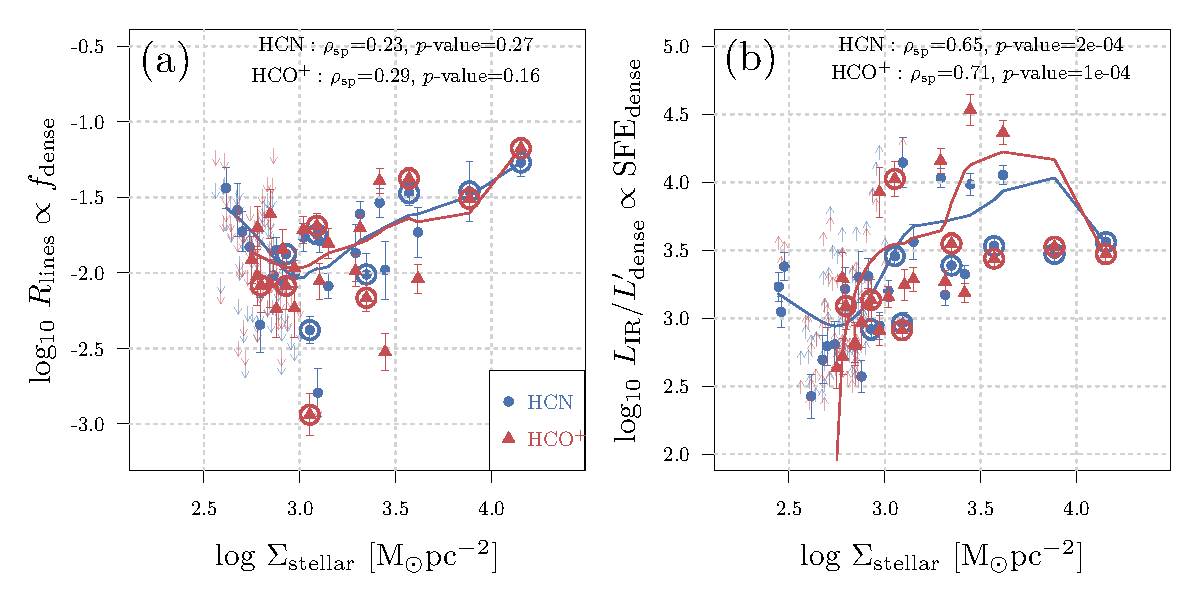
\includegraphics[width=0.99\textwidth]{Jiang_SFE_star.pdf}
\caption{
{\it left:} $f_{\rm dense}$ as a function of stellar surface density \sigmastellar. {\it right:} \sfedense\ as a function of \sigmastellar. These 
two plots explore the effect of stellar components on the dense gas and related
SFE. 
$\rho_\text{sp}$ is the Spearman correlation coefficient and the $p$-value is for the hypothesis test as to whether they have zero correlation. 
The running lines are Local Polynomial Regression fits to guide the eye. The open circles mark those pixels on the major axis of the disk (Jiang et al. submitted). Statistics show that regions with higher \sigmastellar\ tend to have
higher \sfedense.
%\includegraphics[width=0.45\textwidth]{n3628_harp_grid.eps}
%\hskip10pt
%\includegraphics[width=0.45\textwidth]{n253_harp_jiggle.eps}
%
%\caption{The sample schematic diagrams of a grid mode ({\bf left}) and a jiggle
%mode ({\bf right}) observations. The beam width is 13$''$ at 355 GHz and the
%beam spacing is 15$''$ for two points grid pattern observation. For the
%observing mode with 3$\times$3 jiggle pattern that fully sample the nuclear
%region of extended galaxies (e.g.,NGC253/NGC1068/IC342/M82/M83/NGC6946), the
%beam spacing is 10$''$.
} \label{fig:jiang_relation}

\end{figure}

%%%
%\begin{figure}
%\centering
%
%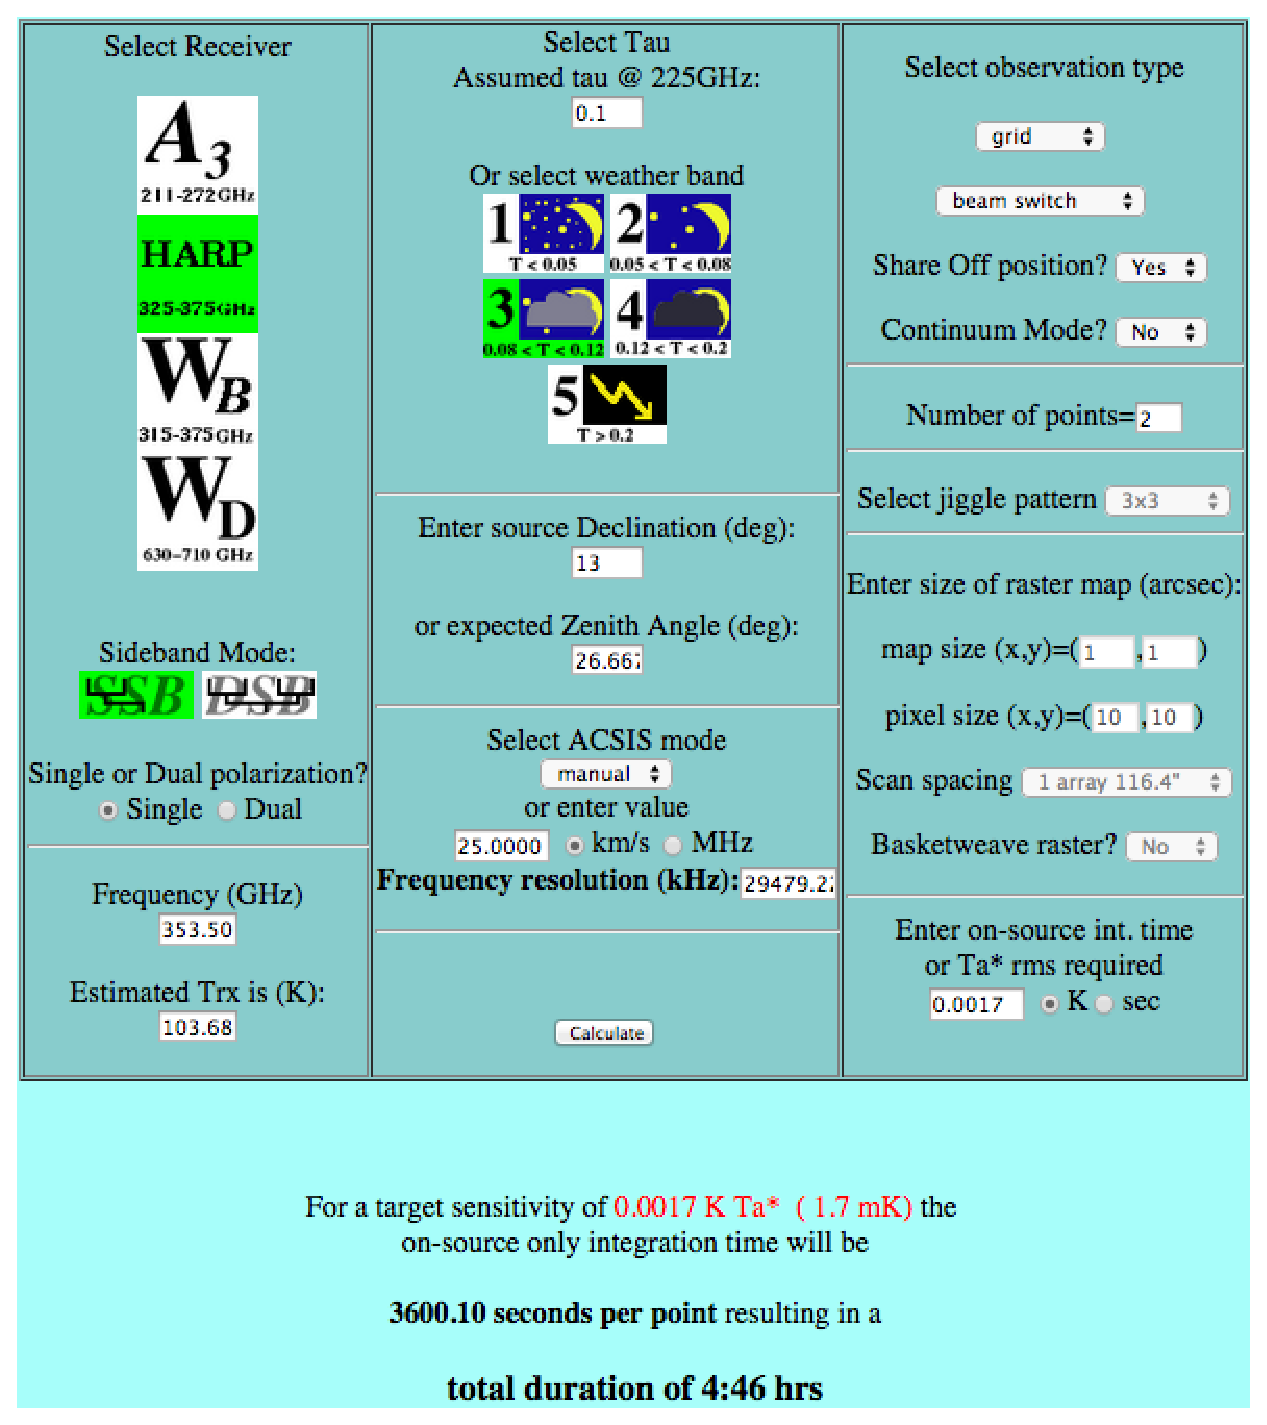
\includegraphics[width=0.45\textwidth]{grid.eps}
%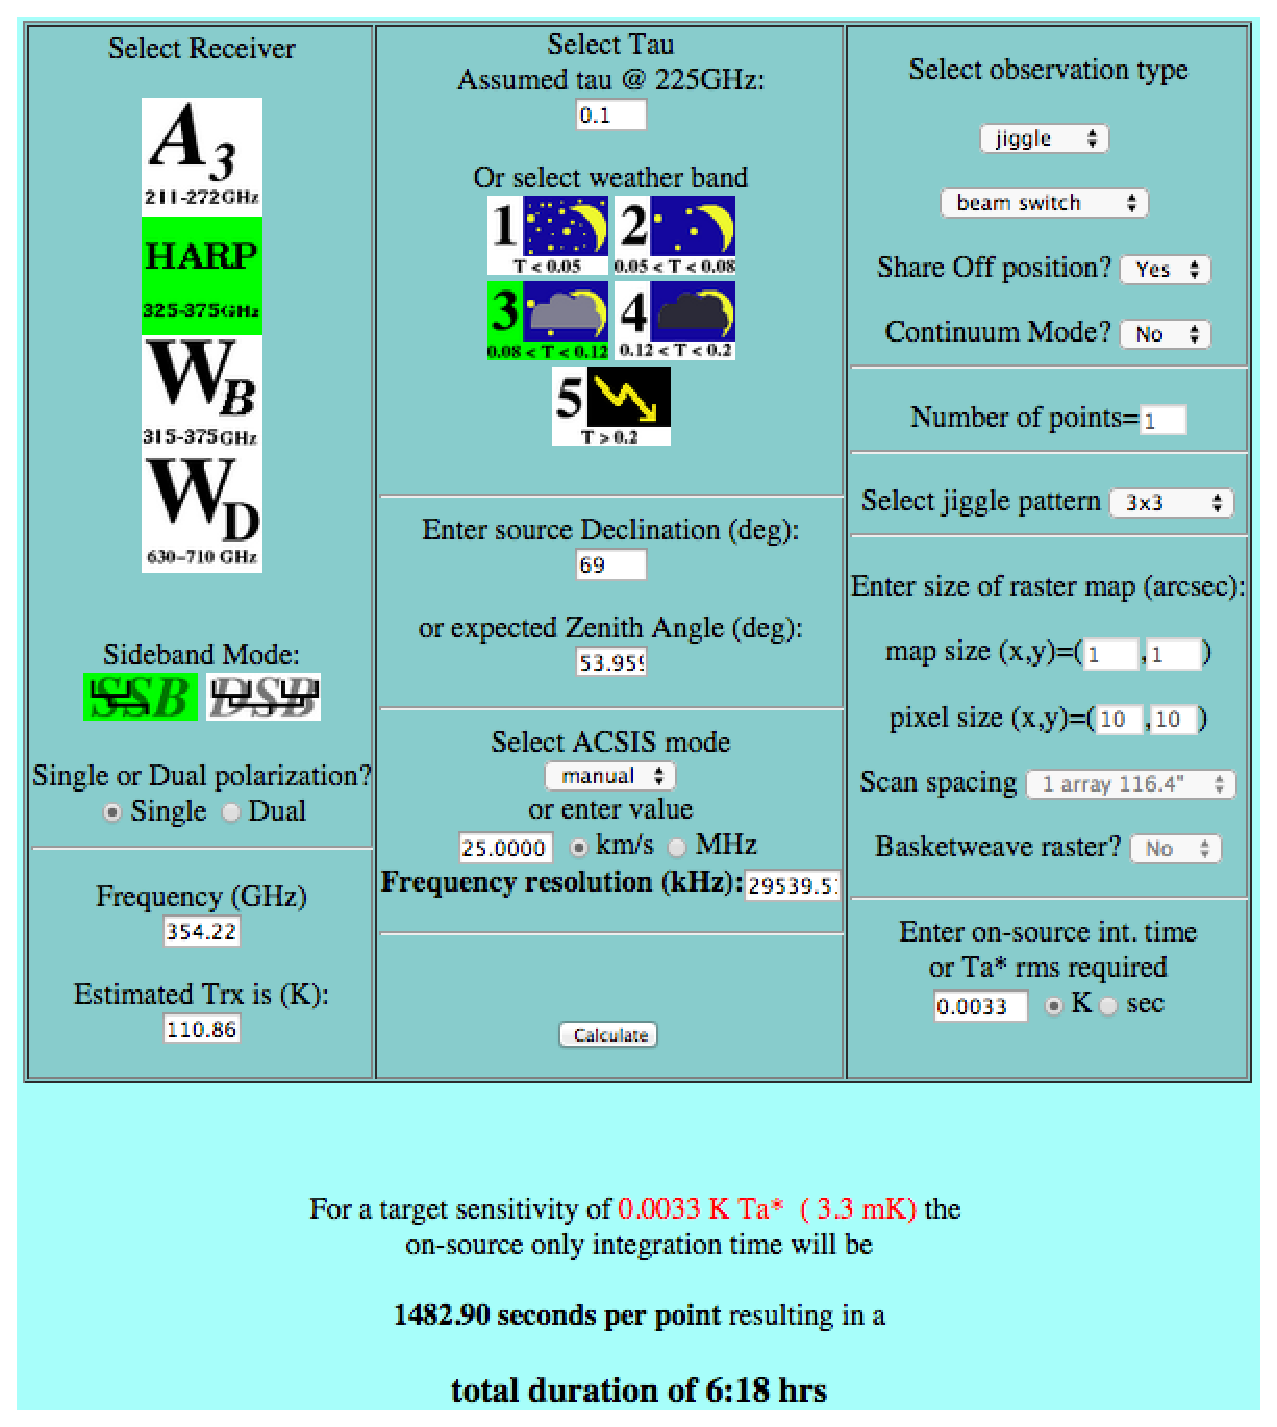
\includegraphics[width=0.455\textwidth]{jiggle.eps}
%
%\caption{Two sample screen grabs of the HiTEC GUI set up.}
%\label{fig:hitec}
%
%\end{figure}





















%\begin{figure}
%\includegraphics[scale=0.4,angle=0]{fig1.eps}
%\includegraphics[scale=0.6,angle=0]{fig2.eps}\\
%\caption{Left: The HCN-FIR correlation (the fit is for local normal galaxies
%with a slope of 1 (open circles)).  Filled circles are high-$z$ AGN/galaxies (Gao et al. 2007)
%and circles with plus signs are local (U)LIRGs.  Right: The correlation between
%$\rm L_{HCN}/L_{CO}$ and $\rm L_{IR}/L_{CO}$ for a local sample (GS04a).}% \label{1}
%\end{figure}
%
%
%\begin{figure}
%\includegraphics[scale=0.3,angle=90]{cs21.eps}
%\includegraphics[scale=0.3,angle=90]{cs32.eps}\\
%\includegraphics[scale=0.3,angle=90]{cs54.eps}
%\includegraphics[scale=0.3,angle=90]{cs76.eps}\\
%\caption{Correlations between the luminosities of CS from $J$=2$\rightarrow 1$
%to  CS $J$=7$\rightarrow$6 and FIR.  For a few nearby galaxies, FIR fluxes were
%measured within the mm telescope beamsizes. The fit lines give slopes of $\sim$
%1.}\label{2} 
%\end{figure}
%
%
%\begin{figure}
%\includegraphics[scale=0.5,angle=-90]{maffei2.eps}
%\caption{ CS $J$=2$\rightarrow 1$ mapping along the major axis of the
%Maffei 2 galaxy.  The unit of x and y axes are both in arcsec. This map
%was taken in less than 2 hours observing time with the IRAM 30-m.  }\label{3}
%\end{figure}
%
%
%
%
%\begin{table}
%        \caption{Sample of CS mapping galaxies }
%\begin{center}
%\begin{tabular}{lllllllcl}
%\hline\hline
%Name      &RA          &DEC        &Diameter     &Tpeak      &Expected Tpeak          &  Time         &  Time \\
%          &J2000       &J2000      &arcmin       & CS(2-1)mK &mK &hrs(weak)          &hrs(strong)\\
%  \hline
%NGC 253        &00:47:33.1 &$-$25:17:18  &27.5     &170       &6,12,50,170,50,12,6   & 4     & 1.5 \\
%NGC 1068       &02:42:40.7 &$-$00:00:48  &7        &30        &8,30,8                & 2     & 0.5 \\
%IC 342         &03:46:48.5 &$+$68:05:46  &21.5     &90        &6,25,90,25,6          & 4     & 0.5 \\
%M 82           &09:55:52.7 &$+$69:40:46  &11.2     &90        &6,25,90,25,6          & 4     & 0.5 \\
%M 83           &13:37:00.9 &$-$29:51:56  &12.9     &40        &10,40,10              & 2     & 0.5 \\
%NGC~6946       &20:34:52.3 &$+$60:09:14  &11.5     &70        &5,18,70,18,5          & 4     & 0.5 \\
%M~51           &13:29:56.2 &$+$47:13:50  &10.42    &70        &6,25,90,25,6          & 4     & 0.5 \\
%%&NGC 3628       &11:20:17.0 &+13:35:23  & 14.8    &10$^a$    &5,20,5                &4.5  \\
%%&NGC 891        &02:22:33.4 &+42:20:57  & 13.5    &15        &4,15,4                &4.5 \\
%%&NGC 2903       &09:32:10.1 &+21:30:03  & 12.6    &15        &4,15,4                & 4.5 \\
%%&NGC 1365       &03:33:36.4 &$-$36:08:25& 11.2    &10$^a$   &5,20,5                & 4.5 \\
%%&NGC 7331       &22:37:04.1 &+34:24:56  & 10.5    &6$^{a}$   &3,12,3                & 4.5  \\
%\hline
%Total          &            &          &         &          &                       & 24  & 4.5 \\
%\hline
%\end{tabular}
%\end{center}
%Notes.  ------ This table contains data of Bayet et al. (2009), and includes
%some results in our former observations.  All the data were taken by IRAM 30-m
%except for NGC~253, which was observed with the SEST 15m.  For details, see the
%Technical Justification.\\
%\end{table}
%
%
%
%\begin{table}
%        \caption{Supplementary Sample of former CS detections}
%\begin{center}
%\begin{tabular}{lllllllcl}
%\hline\hline
%
%Source Name    &RA           &DEC       &Log(Lir) &CS 5$\rightarrow$4  &CS 2$\rightarrow$1   & HCN 1$\rightarrow$0   \\
%               & J(2000)     &J(2000)   &         &(Jy km s$^{-1}$)SMT &(Jy km s$^{-1}$)30m & Jy km s$^{-1}$  \\
%\hline
%NGC~5457       & 14:03:12.5  &$+$54:20:56 &10.20  &                    & 1.8 $\pm$ 0.4$^g$                   &  \\
%NGC~3627       & 11:20:14.9  &$+$12:59:30 &10.38  &                    & 20 $\pm$ 4$^f$          &           \\
%NGC~6090       & 16:11:40.7  &$+$52:27:24 &11.51  & 40 $\pm$ 15$^b$  & &  \\
%NGC~695        & 01:51:14.2  &+22:34:56.5  &11.63   &                    &0.35$\pm$ 0.1       \\
%NGC~6240       & 16:52:58.9  &+02:24:03   &11.85  & 52 $\pm$ 10$^b$        &   needed            &31.2$^d$                    \\
%IRAS~10565+2448& 10:59:18.2  &+24:32:34  &12.02    &                    &3.7 $\pm$0.5 $^b$        &8.6$^c$               \\
%%NGC~4355       & 12:26:54.6  &$-$00:52:39 &10.97  &                    &15.9$\pm$2.5$^a$     &13.0$\pm$1.6   $^a$   \\
%%M~51           & 13:29:55.7  &$+$47:13:53 &10.42  &                    & $<$ 10   $^f$ & \\
%%NGC~6946       & 20:34:52.3  &$+$60:09:14 &10.16  & 60 $\pm$ 5 $^b$        & 11 $\pm$ 6$^f$         & \\
%IRAS~23365+3604& 23:39:01.3  &+36:21:09  &12.13   & 11 $\pm$3.5$^b$  &                     &2.3$^c$             \\
%IRAS~17208-0014  & 17:23:21.9  &-00:17:00.1  &12.39   &                    &1.21 $\pm$ 0.16 \\
%Mrk~231           & 12:56:14.2  &+56:52:26    &12.51   &27$\pm$11 &0.47 $\pm$0.18   \\ 
%\hline
%Total          &            &            &                   9 positions& for weak& CS emission\\
%\hline
%\end{tabular}
%\end{center}
%$^a$ Baan et al. 2008, $^b$ Our observation, $^c$ Gao \& Solomon 2004a,
%$^d$ Graci\'{a}-Carpio et al. 2008, $^e$  Aalto et al. 2002, $^f$ Mauersberg et
%al. 1989, $^g$ Sage et al. 1990 
%\end{table}


\end{document}
